%% bare_jrnl.tex
%% V1.4b
%% 2015/08/26
%% by Michael Shell
%% see http://www.michaelshell.org/
%% for current contact information.
%%
%% This is a skeleton file demonstrating the use of IEEEtran.cls
%% (requires IEEEtran.cls version 1.8b or later) with an IEEE
%% journal paper.
%%
%% Support sites:
%% http://www.michaelshell.org/tex/ieeetran/
%% http://www.ctan.org/pkg/ieeetran
%% and
%% http://www.ieee.org/

\documentclass[journal]{IEEEtran}

\bibliographystyle{IEEEtran}
\usepackage{lineno,hyperref}
\usepackage{amsmath,graphicx, amssymb,tabularx,booktabs}
\usepackage{grffile}
\usepackage{subcaption}
\usepackage[font=small,skip=2pt]{caption}
%\usepackage{boxedminipage}
%\usepackage{algpseudocode}
%\usepackage{algorithm}
\usepackage{xcolor}
\usepackage{comment}
%\usepackage[sort&compress]{natbib}
\usepackage{footnote}
\makesavenoteenv{tabular}

%\setlength{\textfloatsep}{10pt plus 1cm}


% Example definitions.
% --------------------
\def\x{{\mathbf x}}
\def\L{{\cal L}}


% *** GRAPHICS RELATED PACKAGES ***
%
\ifCLASSINFOpdf
  % \usepackage[pdftex]{graphicx}
  % declare the path(s) where your graphic files are
  % \graphicspath{{../pdf/}{../jpeg/}}
  % and their extensions so you won't have to specify these with
  % every instance of \includegraphics
  % \DeclareGraphicsExtensions{.pdf,.jpeg,.png}
\else
  % or other class option (dvipsone, dvipdf, if not using dvips). graphicx
  % will default to the driver specified in the system graphics.cfg if no
  % driver is specified.
  % \usepackage[dvips]{graphicx}
  % declare the path(s) where your graphic files are
  % \graphicspath{{../eps/}}
  % and their extensions so you won't have to specify these with
  % every instance of \includegraphics
  % \DeclareGraphicsExtensions{.eps}
\fi


% correct bad hyphenation here
%\hyphenation{op-tical net-works semi-conduc-tor}


\begin{document}
%
% paper title
% Titles are generally capitalized except for words such as a, an, and, as,
% at, but, by, for, in, nor, of, on, or, the, to and up, which are usually
% not capitalized unless they are the first or last word of the title.
% Linebreaks \\ can be used within to get better formatting as desired.
% Do not put math or special symbols in the title.
\title{Reducing object prior-bias from sparse-projection tomographic reconstructions}
%
%
% author names and IEEE memberships
% note positions of commas and nonbreaking spaces ( ~ ) LaTeX will not break
% a structure at a ~ so this keeps an author's name from being broken across
% two lines.
% use \thanks{} to gain access to the first footnote area
% a separate \thanks must be used for each paragraph as LaTeX2e's \thanks
% was not built to handle multiple paragraphs
%

\author{Preeti Gopal,
  Sharat Chandran,
  Imants Svalbe,
        and~Ajit Rajwade
\thanks{Preeti Gopal is currently with the Applied Artificial Intelligence Institute, Deakin University; p.gopal@deakin.edu.au}
\thanks{Sharat Chandran and Ajit Rajwade are with the Department of Computer Science and Engineering, IIT Bombay; \{sharat, ajitvr\}@cse.iitb.ac.in}
\thanks{Imants Svalbe is with the School of Physics and Astronomy, Monash University; imants.svalbe@monash.edu}}



% make the title area
\maketitle

% As a general rule, do not put math, special symbols or citations
% in the abstract or keywords.
\begin{abstract}
  Tomographic reconstruction from undersampled measurements is a
  necessity when the measurement process is potentially harmful, needs
  to be rapid, or is resource-expensive. In such cases, information
  from previously existing longitudinal scans of the same object
  (`object-prior') helps in the reconstruction of the current object
  (`test') from its significantly fewer measurements. A common problem
  with these techniques is the %strong 
  influence of object-priors in
  the reconstruction of new changes in the test.  In this work, we
  mitigate this problem by first estimating the location of changes (`new
  regions') and then imposing object-prior in \textit{only} those regions
  which are similar to the prior (`old regions').

  Our work is based on longitudinal data acquisition scenarios where
  we wish to study new changes that evolve within an object over time,
  such as in repeated scanning for disease monitoring, or in
  tomography-guided surgical procedures. While reconstruction is easily feasible
  when measurements are acquired from a large number of projection
  angles (`views'), it is challenging when the number of views is
  limited (sub-Nyquist). We show that in the latter case, a
  `spatially-varying' technique is appropriate in order to prevent the
  prior from adversely affecting the reconstruction of new structures
  that are absent in any of the earlier scans. The reconstruction of
  new regions is safeguarded from the bias of the prior by computing
  regional weights that moderate the local influence of the priors. We
  are thus able to effectively reconstruct both the old and the new
  structures in the test. We have tested the efficacy of our method on
  synthetic as well as real projection data, in both 2D and 3D. Our
  technique significantly improves the overall quality of
  reconstructions while minimizing the number of measurements needed
  for imaging in longitudinal studies.% We show that with   as little as $2\%$ of measurements, our method achieves a structural   fidelity of $0.84$, with $1.00$ representing ideal reconstruction.
\end{abstract}

% Note that keywords are not normally used for peerreview papers.
\begin{IEEEkeywords}
Limited-view tomographic reconstruction, regularization priors, object priors, longitudinal studies.
\end{IEEEkeywords}


% For peer review papers, you can put extra information on the cover
% page as needed:
% \ifCLASSOPTIONpeerreview
% \begin{center} \bfseries EDICS Category: 3-BBND \end{center}
% \fi
%
% For peerreview papers, this IEEEtran command inserts a page break and
% creates the second title. It will be ignored for other modes.
\IEEEpeerreviewmaketitle



\section{Introduction}
\label{sec:intro}
Computed Tomography (CT) deals with the recovery of details of an
object's interior from a limited set of projection data acquired by
passing X-rays at different orientations (`views'). It is preferable
to minimize the radiation exposed in order to prevent any potential
damage to it and in order to reduce the acquisition time. Therefore,
current research seeks to either significantly reduce the radiation
intensity required to reconstruct with adequate
fidelity~\cite{yang2018,Lin2016,Xie2017,gopal2019low} or significantly
reduce measurements required to reconstruct with
adequate fidelity. For the latter case, there are two lines of
pursuit. One is to intelligently choose those sets of projection views
that capture most
information~\cite{King2018,Anthony2018,barkan17,fischer16,andrei14},
and the other, which is the focus of this paper, is to design the
reconstruction algorithm in order to achieve the most accurate
recovery of the underlying slice, given the measurements from any
limited set of views~\cite{yang2018,geyer2015,kilic2011}.

In conventional data acquisition techniques, tomographic measurements
$\boldsymbol{y}$ are acquired by sampling the physical object
$\boldsymbol{x}$ uniformly with a substantial number of views, ideally
above the Nyquist rate. In such a case when there are sufficient
measurements, reconstruction using conventional filtered
backprojection (FBP) suffices, as seen in Fig.~\ref{fig:story} (first
column, 800 views). The figure shows the ground truth image
(260$\times$260) of naturally growing sprouts at the top left (the
details of this dataset are postponed to Section~\ref{sec:datasets}).

However, reconstruction from reduced views has been made possible by
assuming the data to exhibit certain properties such as smoothness in
image space~\cite{Essam2015}, sparsity in gradient space~\cite{TV} or sparsity under
certain mathematical transforms~\cite{Donoho,introCS} such as the
Discrete Cosine Transform (DCT).  There are multiple such
regularization priors such as the Compressed
Sensing based l1-ls prior~\cite{my_dicta_paper}. For the purposes of
demonstrating the efficacy of our method, we use the well known Total Variation (TV)
regularization prior.
If $\boldsymbol{\mathcal{R}}$ represents the acquisition
model, then the TV-regularized solution is described by one that
minimizes a combination of least squares error and the $TV$-norm of
the object $\boldsymbol{x}$. Mathematically, we choose to minimize
$J_{TV}(\boldsymbol{x})$ where

 \begin{equation}
   J_{TV}(\boldsymbol{x}) = \lVert\boldsymbol{\mathcal{R}x}- \boldsymbol{y}\rVert_2^2 + \lambda_{TV}TV(\boldsymbol{x})
   \label{Eq:simple_TV}
 \end{equation}

 % where the $TV$-norm is given by
 and 

  \begin{equation}
   TV(\boldsymbol{x}) = \sum_{i,j}\nabla_{ij}(\boldsymbol{x}),
   \label{Eq:definition_TV}
\end{equation}

  where $\nabla$ represents the gradient operator.
  
 Fig.~\ref{fig:story} (second column) demonstrates the benefit of
 using a regularization prior when the number of projection views is
 limited (for example reducing sampling to 100 views for the same resolution reconstructed image).  We solve this cost function using an optimal
 first-order method for large-scale TV regularization presented
 in~\cite{TVReg} and available in~\cite{TVReg-lib}.

 %%% Postpone later We observed that there was no significant benefit
 %%% in choosing wavelets over DCT.  }

 \begin{figure}[t]
\centering
	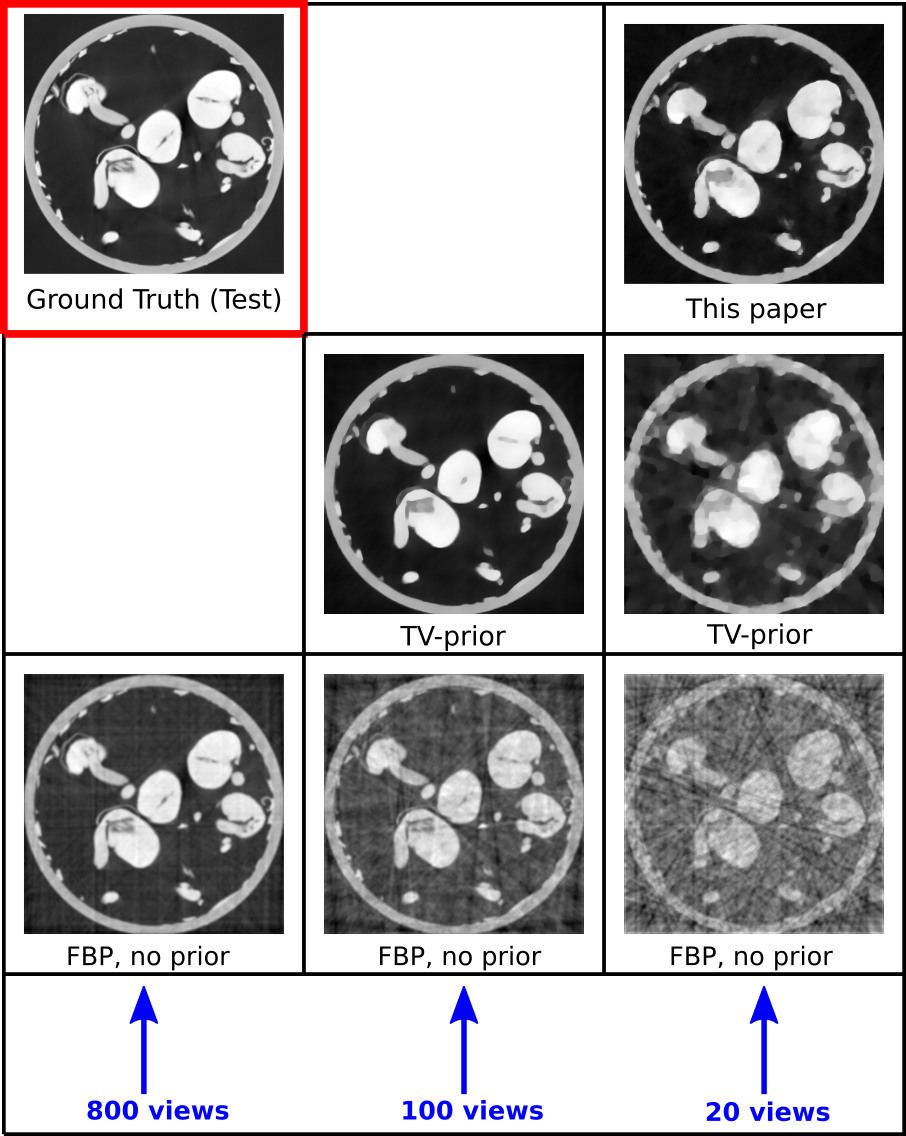
\includegraphics[width=0.45\textwidth]{../images/story/post_TCI/story.png}
        \caption{Illustration of the use of priors in reconstruction
          as the number of views reduces. For all cases, the ground
          truth (260$\times$260) appears in the top left.  For
          extremely large number of views (800 views), the standard
          FBP reconstruction (first column) is of very good quality
          (Structural Similarity Index Metric, SSIM=0.92, ideal SSIM=1.00). As the
          number of views become limited (100 views), reconstruction
          using the Total Variation regularization prior (TV, middle
          column) is better both visually and quantitatively than FBP
          (SSIM of 0.96 vs 0.82). If the number of views is
          drastically reduced (20 views), the presence of both TV
          prior and object-prior together with the spatially-varying
          technique of this paper improves the reconstruction
          (SSIM=0.91) when compared to presence of TV-only prior
          (SSIM=0.87) or no prior (SSIM=0.64).
          % , an improvement by $4\%$ and $27\%$ respectively (since the ideal SSIM=1)
}
 \label{fig:story}
 \end{figure} 

 When the number of views is reduced significantly further (as
 discussed in this work), a regularization prior alone is not
 sufficient.  In such cases additional information (`object-prior')
 specific to the current object being scanned (called the `test'
 henceforth) is useful in further improving the reconstruction.  While
 this has been done in the context of dynamic CT-scans (discussed more
 in Section~\ref{sec:related}), in this paper we use a set $S$ of
 previous scans of the same object. This is relevant in a longitudinal
 context: the acquisition of sequential CT scans of the same subject
 in order to track time-evolving changes within the subject's
 interior.
 \subsection{Difficulties}
 
 With the use of an object-prior, a \emph{new} challenge emerges. The prior
 set $S$ may potentially overwhelm the necessary details~\cite{mythesis}, and when
 several prior scans are available, finding the best one is an
 issue. We therefore devise an algorithm that estimates the location
 and magnitude of new changes in the (unknown) test. As we show in
 Section~\ref{sec:method_spatially_varying_prior}, this prevents the prior from adversely affecting the reconstruction of new
 regions in the test. We refer to this method as a
 \textit{spatially-varying} prior-based reconstruction routine, that
 still uses \textit{all} the previous scans in the set $S$, without
 using any of the prior scans \textit{as is}, or endeavoring to choose
 one ``right'' prior. In this way, this work is novel and to be
 contrasted with 
 earlier work. As seen in Fig.~\ref{fig:story} (last column, 20
 views) our method uses the set $S$ to yield a better reconstruction
 than the regularization-only, or the backprojection-only methods.

 \subsection{Paper organization}
 This paper is organized as follows. After discussing related work in
 Section~\ref{sec:related}, Section~\ref{sec:contributions} lays down
 the \emph{key contributions} of this work.
 
Most datasets from commercial scanners do not provide raw
measurements. In order to validate our method quantitatively, we
created new cone-beam longitudinal CT datasets, details of which are
described in Section~\ref{sec:datasets} -- these will be offered to
the community in the public domain.  (In addition,
Section~\ref{sec:tmh} demonstrates the utility of our method on a
longitudinal medical dataset involving the liver in a radio-ablation
study.)
 
We now move to the
details. Section~\ref{sec:method_spatially_varying_prior} describes
the computation of a spatially-varying weights map in order to preserve
new changes in the test.  Results are presented in
Section~\ref{sec:results_spatially_varying_prior}. Section~\ref{sec:discussion}
discusses tuning of the hyperparameters involved. %and limitations of
 %our method.
 Finally, we conclude with key inferences that can be
 drawn from our work in Section~\ref{sec:conclusions}.
% We present results on real and simulated 3D
%  data for different longitudinal studies.  These are studies wherein
%  sequential CT scans of the same object are acquired to track
%  time-evolving changes within its interior.
 
  %although this optimizer removes most of the artefacts created due
  %to sub-sampling, its reconstruction is blurred when the number of
  %views is very limited, as shown in Fig.~\ref{fig:story2}.
%(2) there is the key issue of the choice of \textit{a particular} previously scanned object as template among the many previously acquired scans

 \section{Related Work}
 \label{sec:related}
 The idea of using a reduced number of views is most pronounced in
 specialized applications. For example, in~\cite{Essam2015},
 sparsity-constrained optimization is presented for angiography. Here,
 the regions of interest are the vessels alone and they are
 highlighted by physically inserting a contrast agent, and therefore
 there is an inherent sharper contrast between the vessels and the
 background.  In other applications where the spatial-gradient of the
 underlying volume is known to be sparse, the `total variation'
 method, as used in~\cite{Li2015,Polak2017}, can be applied.  However,
 as shown earlier in Fig.~\ref{fig:story}, these regularization priors
 are not sufficient when very few views are acquired, thus needing
 information from stronger priors such as those obtained from previous
 scans of the same or similar object.

%  As can be seen
% in the situatiowe will
% later see in Figs.\ref{fig:object-prior_test_okra}
% and~\ref{fig:object-prior_test_sprouts}, the spatial-gradient of many
% datasets is not sparse.

Most object-prior based reconstruction have been in the areas of
dynamic CT and 4D-CT. %In dynamic CT, the object being scanned
%undergoes changes between successive projection views and hence is not
%stationary even within a single complete scan. In contrast, in 4D-CT,
%a set of 3D CT scans are taken over short intervals of time, and the
%object undergoes changes between successive scans.  The reconstruction
%is then performed over the entire set generating several 3D
%volumes.
%In most scenarios, the object-prior
The object-prior usually consists of an object reconstructed to high
quality from a large number of projection angles. One of the earliest
pieces of work in this area is the well-cited PICCS
method~\cite{PICCS} for dynamic CT, which enforces a robust-norm based
similarity between the test and the object prior, in addition to a
sparsity prior on the test. Its limitation is the unchecked
over-emphasis of the prior on the reconstruction of the test at
hand. A closely related method called PIRPLE was proposed
in~\cite{pirple}, with additional steps to register the object prior
and the test and a somewhat more flexible combination of data fidelity
terms, sparsity prior and object prior. However, this method too has
similar limitations as PICCS.

In order to prevent the object-prior from overwhelming the
reconstruction of test, a few other approaches have either estimated
the motion between the object-prior and the test or have applied very
specific object-properties for identifying new changes in test.
Examples for the former include~\cite{koen2020}, where changes across
the successive scan volumes are assumed to be continuous, thus
enabling the use of optical flow to model the motion between
corresponding voxels of different scan volumes. In another
study~\cite{vincent2017}, changes between successive scans were
modeled by affine deformation whose parameters were computed for
motion-correction, which in turn enables acquisition from fewer
views. In~\cite{daniil2015}, all the scan volumes are reconstructed
together using spatio-temporal regularization. Here again, the
inherent assumption is the continuity across volumes in space or time.

The methods that use object-specific knowledge are~\cite{Van2015}
and~\cite{Marjolein2016}.  In~\cite{Van2015}, knowledge of attenuation
coefficient of the fluid is used as a prior for reconstructing its
flow through gravel. However, this relies on additional expert domain
knowledge which may not be available or which may be infeasible to
acquire. Other approaches variously use robust principal components
analysis assuming that the object consists of a large static part
(background) and a sparse moving part (foreground)~\cite{HaoGao} or
spline-based models for tracking the regions of change in an SIRT
framework~\cite{Van2014}.

All of these
techniques~\cite{daniil2015,koen2020,Van2015,HaoGao,Van2014}
essentially reconstruct all the different stages of the object
\textit{simultaneously}, and use the extra redundancy across time
simultaneously. In the scenario of a longitudinal study (where
projection measurements are acquired at instants that are several
weeks apart) which we consider in this paper, such approaches are not
feasible. A longitudinal study will necessarily require
reconstructions soon after acquisition of each set of measurements.

There also exist methods for estimating new changes (in the test)
directly in projection space. In such techniques which can be used in
longitudinal studies, the object-prior is projected in the same set of
views as the current set of test measurements, and a set of projection
differences is computed. These projection differences are essentially
tomographic projections of differences between the unknown test and
the known object-prior. Hence, a variety of reconstruction algorithms
can be used to estimate such a difference image which can then be
added to the object-prior to yield the final estimate of the
test. Such methods have been proposed
in~\cite{Pourmorteza2015,Lee2012}. However, reconstruction of the
difference image will inherently contain sub-sampling artefacts, and
these artefacts will appear in the final reconstruction as there is no
mechanism to mitigate them (unlike the method that we propose). %This
%can be seen in Sec.~4 of our supplementary material~\cite{supp_paper},
%where we have compared our method with~\cite{Lee2012}.


In this paper, we present a technique that makes use of multiple
object priors, corresponding to high quality reconstructions of
similar objects across time, typically in a longitudinal study.  We
use these priors to improve the reconstruction of the test from
largely undersampled measurements. In particular, we define regions of
change between the test and the eigenspace spanned by previous high
quality object-priors in a purely data driven manner. Additionally,
our technique differentiates between genuine structural changes and
``changes'' that appear due to undersampling artefacts.  Besides this,
since we use a statistical model with multiple object-priors, we avoid
the problem of selecting an appropriate single object-prior
unlike~\cite{PICCS,Pourmorteza2015,Lee2012,pirple,Marjolein2016} and
also make use of the additional information available in multiple
priors. Our technique also has the advantage of not requiring any
expert-domain knowledge about the object being scanned.

 In the recent past, deep learning based techniques have also been widely used for limited view CT reconstruction without the use of any longitudinal object-prior. For example, in~\cite{anirudh}, a neural network is trained to predict the complete sinogram from an incomplete one obtained from few-view imaging. This complete sinogram is then fed to analytical reconstruction algorithms to obtain the final reconstruction. Hence, one may in principle use this full sinogram as an alternate initial reconstruction of the test within our framework. \cite{bo2021} presented a cascade of neural networks that predict full-view reconstruction from limited view FBP reconstruction while simlutaneously ensuring consistency between the predicted sinugram and the acquired sinogram. \cite{special} trains an adverserial network for artifact removal and edge preservation in limited view reconstruction. While all of the above methods predict full-view reconstruction from the measurements of test object alone, we believe it is beneficial to use information from longitudinal data, especially if naturally available, like in the radio-frequency ablation datasets that we use. In this context, we present an analytical method that uses the available longitudinal data to better inform the reconstruction of the test. We first construct a `weights map' that gives clear insights about regions of change within the object over time.  
 
%-------------------------------------------------------------------

\section{Contributions}
\label{sec:contributions}
This paper focuses on few-views reconstruction with an emphasis on
longitudinal studies. In contrast to the object-prior based studies
mentioned above, we reconstruct the current test object without any
assumption of continuity of changes or knowledge of the attenuation
coefficients of the structures. We also do not make any temporal
assumption in terms of time intervals -- prior scans could be months
apart which is typical in cancer scanning, or could be a few
minutes/seconds apart which is typical in CT-guided surgeries. We use
the current measurements from few-views and previous scans of the same
object.

A key idea in our work is this starting
point -- the new test volume is close to the space spanned by the
eigenvectors of multiple representative previously scanned objects.
We then present a method to accommodate new changes in the test that
may lie outside of this eigenspace. This will prevent an unnecessary
bias when reconstructing the data. As a solution, our method moderates
the control of the prior by estimating and imposing spatially-varying
weights to the prior in order to reconstruct new structures
accurately. This spatially-varying prior tunes the effect of the
templates in different regions of reconstruction.

Fig.~\ref{fig:prior_overview} provides an overview.

 %Various forms of object priors have been used for reconstruction from limited views (`few-views'). In ~\cite{Van2014}, the time-varying region within an object is computed by modelling it as a B-spline.
% \cite{PICCS} uses only a single template and enforces a uniform similarity between the current object's reconstruction and the single template. 
%In addition, when some extra information about the object's structure is known~\cite{PICCS,cardiacPICCS,lubner2011,pirple,mota2017},   %The latter limitation was relaxed in~\cite{liu2016,Xu2012} by building dictionary-based priors from multiple previously scanned objects. However, as reported in~\cite{my_dicta_paper}, dictionary priors are not as accurate and fast as global eigenspace priors.

 \begin{figure}[h]
\centering
	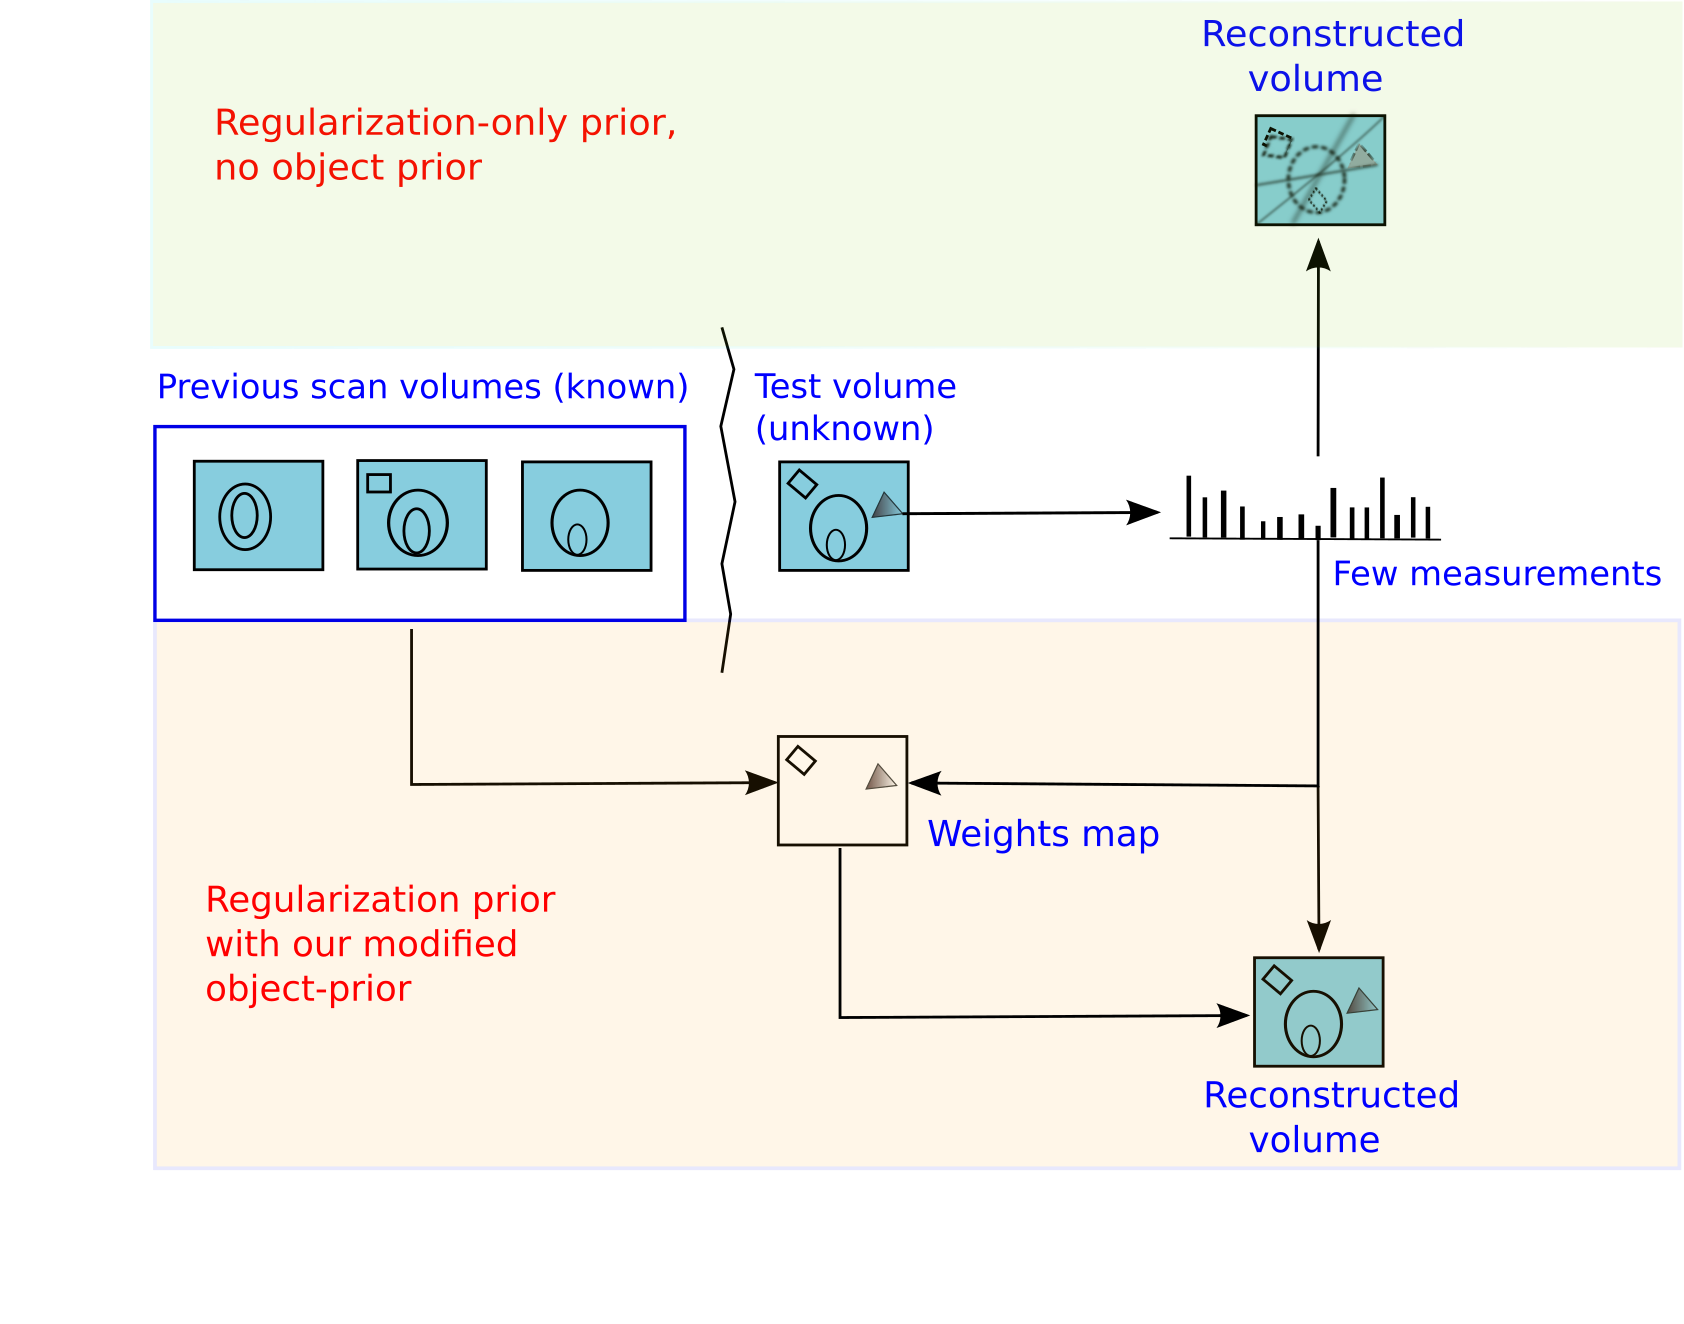
\includegraphics[width=0.5\textwidth]{../images/prior_cmb.png}
        \caption{Overview of our work. (Upper) When the number of
          measurements is vastly lower than what is conventionally
          used (last column of Fig.~\ref{fig:story}) a regularization
          prior such as Total Variation alone is not sufficient to
          mitigate the sub-sampling artefacts. (Lower) An object-prior
          must be used to provide additional information, but in
          addition, new bias should not be introduced. To this end,
          here we propose using a spatially-varying weights-map to
          modulate the effect of object-prior on the final
          reconstruction.}
 \label{fig:prior_overview}
\end{figure}

In summary, the key contributions are
\begin{itemize}
\item We create new 3D biological datasets (Section~\ref{sec:datasets}) and
  present results on real cone-beam projections. Our datasets and code
  will be made available to the community.
  \item We design a weights-map
    to depict the location and strength of new changes in the test at
    every voxel. A novel algorithm is presented to build this map from
    sub-sampled measurements of the test and a set of high quality
    templates. Once the weights-map is built, it is used for accurate
    reconstruction of those changes in the test that are absent in all
    of the templates. Results appear in
    Section~\ref{sec:results_spatially_varying_prior}.
  \item We show the efficacy of our results in a real-life medical
    longitudinal study with data obtained in a clinical setting from
    a live teaching and
    research hospital.
\end{itemize}
While we demonstrate our results with a Total Variation regularization
prior, this work provides a technique that can improve upon any chosen
baseline reconstruction when measurements are extremely sparse.  


%-------------------------------Dataset----------------------------
\section{Datasets}
\label{sec:datasets}
In this section, we present details of the biological and medical
datasets created and used for this work. For the first two datasets
namely, Potato and Okra, the raw measurements and corresponding
parameters for cone-beam imaging model are available to us.  Hence all
reconstructions on these datasets were performed directly from real
projection measurements. These datasets are ``Type A'' datasets in the
description below.  For the other two datasets (Type B), namely,
Sprouts and Liver, the raw measurements and the parameters of imaging
model were not available to us (due to propriety concerns) and hence
only reconstructed volumes of real data were at hand; we therefore
generated measurements from these datasets assuming a circular
cone-beam imaging model for 3D and a parallel-beam imaging model for
2D.

In each case, we remark on the design of the choice of the test chosen
in the dataset.

\subsection{Datasets with the imaging model available}
\label{sec:potatoAndOkra}

These consist of longitudinal scans of a Potato and an Okra, both
acquired by the first author at the Australian National University
(ANU). 

\textbf{Potato:} This dataset consisted of four scans of the humble
potato (Fig.~\ref{fig:potato_dataset}). While the first
scan was taken of the undistorted potato, subsequent scans were taken
of the same specimen, each time after drilling a new hole halfway into
the potato. Measurements from each scan consisted of real circular
cone-beam projections from 900 views, each of size
150$\times$150. %Further, this alignment can be refined following
%every update of the reconstructed test volume.
In our experiments,
the first 3 volumes were used to build the object-prior and the last
volume was used as the test. The ground truth consists of volumes of
size 150$\times$150$\times$100 reconstructed using the 
Feldkamp-Davis-Kress (FDK) from the full
set of 900 projection views.
%---------------------------------------
\begin{figure}[!h]
    \begin{subfigure}[b]{0.24\linewidth}
        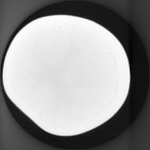
\includegraphics[width=\textwidth]{../images/potato/template_1.png}
\captionsetup{labelformat=empty}       
 \caption{}
    \end{subfigure}
    \begin{subfigure}[b]{0.24\linewidth}
        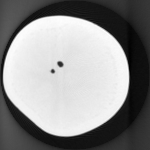
\includegraphics[width=\textwidth]{../images/potato/template_2.png}
\captionsetup{labelformat=empty}
        \caption{}
     \end{subfigure}
    \begin{subfigure}[b]{0.24\linewidth}
        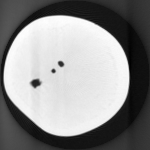
\includegraphics[width=\textwidth]{../images/potato/template_3.png}
\captionsetup{labelformat=empty}
        \caption{}
     \end{subfigure}
    \begin{subfigure}[b]{0.235\linewidth}
        \fcolorbox{white}{blue}{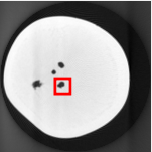
\includegraphics[width=\textwidth]{../images/potato/testIm_color.png}}
\captionsetup{labelformat=empty}
\caption{}
\label{fig:potato3D_test}
     \end{subfigure}
      \caption{Potato 3D dataset: One slice each from the scanned
        objects that are used as templates (the first three from
        left) and a slice from the test volume (extreme right). Notice
        the appearance of the fourth hole in the test slice. 3D visualization is available
      in the supplementary material~\cite{supp_paper}.}
\label{fig:potato_dataset}
\end{figure}

\textit{Remark:} The test slice (unlike the Okra below) was designed
to show the presence of a new feature (last picture in
Fig.~\ref{fig:potato_dataset}. Although the potato is visually bland,
paradoxically, this becomes the reason that the Potato is challenging
if a new method has to be shown to be effective.  Simpler methods may
suffice.  Nevertheless, we show superior performance with our method by
vastly reducing the number of measurements corresponding to the ground truth.



 \textbf{Okra:} This dataset is that of an Okra specimen consisting of
 its five scans (Fig.~\ref{fig:object-prior_test_okra}). Each of the
 scanned volumes consists of a varying number of cuts (or
 deformations) on the surface of the specimen. The specimen was kept
 in the same position throughout the acquisitions. Measurements
 consisted of real circular cone-beam projections from 450 views, each
 of size 336$\times$156.
%In cases where such an
%alignment is not present, all the template volumes must be pre-aligned
%before computing the eigenspace. The test must be registered to the
%object-prior after its preliminary pilot reconstruction.
In our experiments, the first 4 volumes shown in
Fig.~\ref{fig:object-prior_test_okra} were used to build the
object-prior and the last volume was used as the test. Note that in
the region marked red, all the templates have a deformation, and hence
an unchecked reliance of object-prior for the reconstruction of test
in this region will result in a deformation. The ground truth consists
of volumes of size 338$\times$338$\times$123 reconstructed using the
FDK algorithm~\cite{FDK} from the full set of
450 view projections.  

 %--------------------------------okra data-------------------------------
\begin{figure}[!h]
  \begin{subfigure}[b]{0.18\linewidth}
        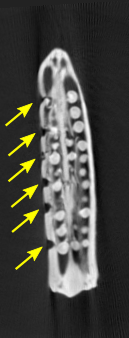
\includegraphics[width=\textwidth]{../images/okra/template4_marked.png}
\captionsetup{labelformat=empty}
        \caption{}
  \end{subfigure}
  \begin{subfigure}[b]{0.18\linewidth}
        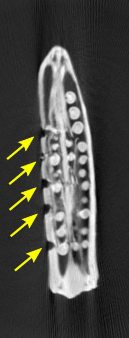
\includegraphics[width=\textwidth]{../images/okra/template3_marked.png}
\captionsetup{labelformat=empty}
        \caption{}
     \end{subfigure}
    \begin{subfigure}[b]{0.18\linewidth}
        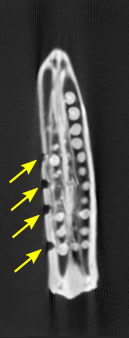
\includegraphics[width=\textwidth]{../images/okra/template2_marked.png}
\captionsetup{labelformat=empty}
        \caption{}
    \end{subfigure}
     \begin{subfigure}[b]{0.18\linewidth}
        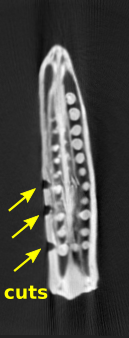
\includegraphics[width=\textwidth]{../images/okra/template1_marked.png}
\captionsetup{labelformat=empty}       
 \caption{}
    \end{subfigure}
     \begin{subfigure}[b]{0.148\linewidth}
        \fcolorbox{white}{cyan}{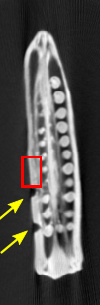
\includegraphics[width=\textwidth]{../images/okra/post_TCI/test_marked.png}}
\captionsetup{labelformat=empty}
        \caption{}
    \end{subfigure}
     \caption{Okra 3D dataset: One slice each from the scanned objects
       that are used as templates (the first four from left) and a
       slice from the test volume (extreme right). Notice the region
       marked in red box; while all slices have deformities here, the
       test has none.}
\label{fig:object-prior_test_okra}
\end{figure}

\textit{Remark:} Unlike the potato, the test was designed as one with
the absence of a feature.  Although mathematically one is the
conjugate of the other, in practice, experimental methods may have
difficulties which explains the choice of our test. Notice also that
the structure of the Okra is intricate as compared to Potato, and this
brings with it a different challenge.



\subsection{Datasets without the imaging model}
These consist of longitudinal scans of a portion of a liver obtained
from Tata Memorial Centre (TMC) ~\cite{tmh} in Parel, Mumbai, and
longitudinal scans of Sprouts obtained from Australian National
University.

 \textbf{Liver:} %We have used this dataset
 %to illustrate an application
%where \textit{both} uniform and spatially-varying priors are
%useful.
TMC is the national comprehensive centre for the prevention,
treatment, education and research in cancer, and is recognized as one
of the leading cancer centres in India. The dataset
(Fig.~\ref{fig:RFA2_test_object-prior}) from this longitudinal medical
study consists of 7 scans taken at different stages of radio-frequency
ablation (RFA) study of a liver. In such a procedure~\cite{Dong2015}, the
physician inserts a thin needle-like probe into the organ. Repeated CT
scans of the patient are acquired in order to track the movement of
the needle and to ensure that it is reaching the appropriate target
tumor. Once the needle hits the tumor, a high-frequency electric
current is passed through the tip of the probe and this burns the
malignant tumor (ablation).  A fairly high amount of radiation is administered to a patient in this RFA procedure~\cite{radiation_dose_RFA}, and hence reducing radiation per scan is highly beneficial here.

In our experiments, we generate parallel beam measurements from 2D
slices from each of the 7 volumes. Note that all these 7 slices are
located at the \emph{same} index (slice number corresponding to the
same depth) within each of the respective volumes.  Observe (in
Fig.~\ref{fig:RFA2_test_object-prior}) that the needle is seen in all
of the 7 slices.
%In our experiments using this dataset, we demonstrate the usefulness of \textit{both} uniform prior and spatially varying prior. For the first case, we choose the first 6 slices to build the object prior and use slice 7 as the test. For the latter case, we choose the first 7 slices to build the object prior and use slice 8 as the test.
%--------------------------Results on TMH data--------------------------
%------------------RFA 2 data
\begin{figure}[h!]
    \begin{subfigure}[b]{0.24\linewidth}
        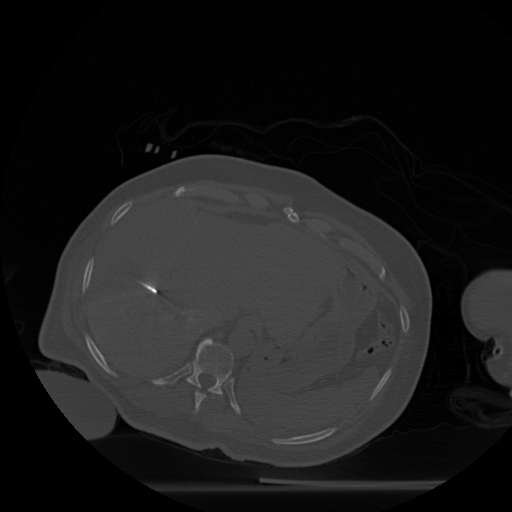
\includegraphics[width=\textwidth]{../images/tmh/RFA2/template1.png}
%\captionsetup{labelformat=empty}       
 \caption{slice 1}
    \end{subfigure}
    \begin{subfigure}[b]{0.24\linewidth}
        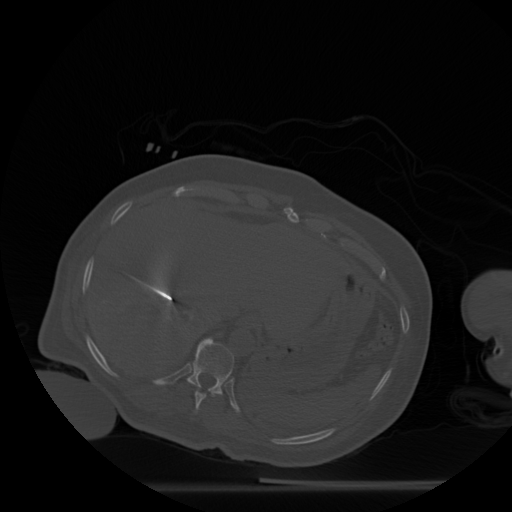
\includegraphics[width=\textwidth]{../images/tmh/RFA2/template2.png}
%\captionsetup{labelformat=empty}       
 \caption{slice 2}
    \end{subfigure}
     \begin{subfigure}[b]{0.24\linewidth}
        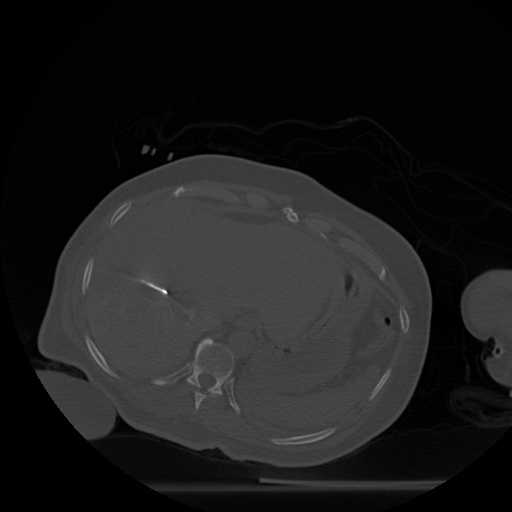
\includegraphics[width=\textwidth]{../images/tmh/RFA2/template3.png}
%\captionsetup{labelformat=empty}       
 \caption{slice 3}
    \end{subfigure}
       \begin{subfigure}[b]{0.24\linewidth}
        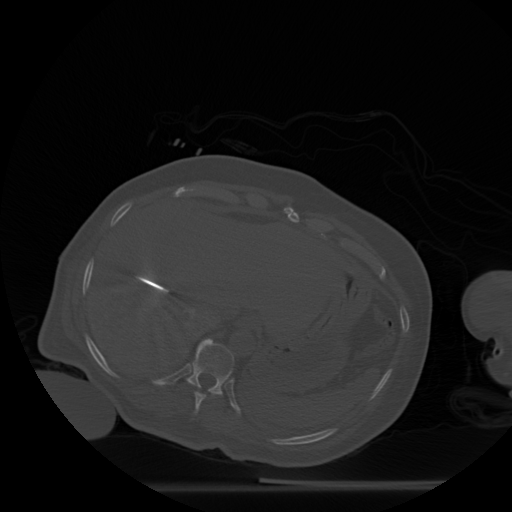
\includegraphics[width=\textwidth]{../images/tmh/RFA2/template4.png}
%\captionsetup{labelformat=empty}       
 \caption{slice 4}
    \end{subfigure}
       \begin{subfigure}[b]{0.24\linewidth}
        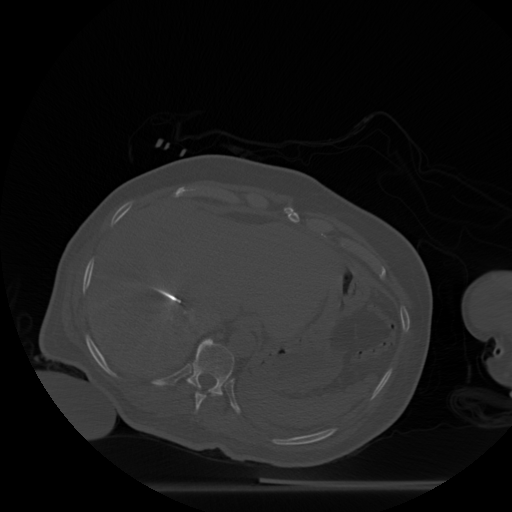
\includegraphics[width=\textwidth]{../images/tmh/RFA2/template5.png}
%\captionsetup{labelformat=empty}       
 \caption{slice 5}
    \end{subfigure}
              \begin{subfigure}[b]{0.24\linewidth}
        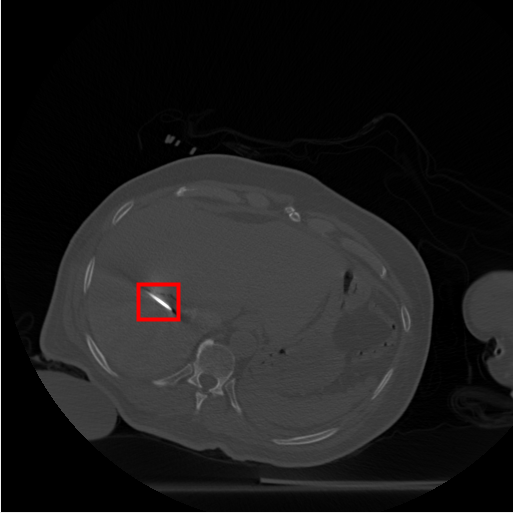
\includegraphics[width=\textwidth]{../images/tmh/RFA2/template6_color.png}
%\captionsetup{labelformat=empty}       
 \caption{slice 6}
    \end{subfigure}
       \begin{subfigure}[b]{0.23\linewidth}
        \fcolorbox{white}{green}{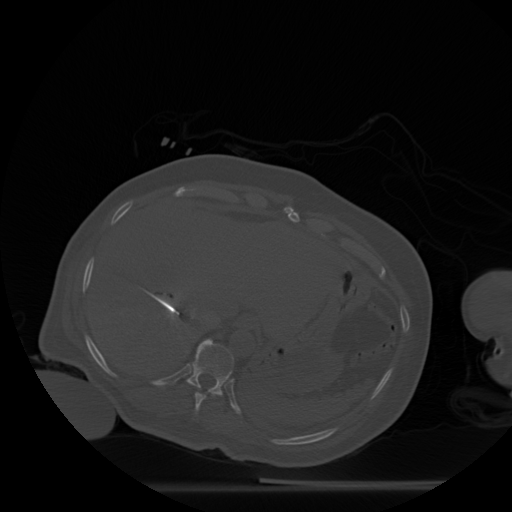
\includegraphics[width=\textwidth]{../images/tmh/RFA2/template7.png}}
%\captionsetup{labelformat=empty}       
 \caption{slice 7 (test)}
    \end{subfigure}     
     \caption{Radio-frequency ablation dataset: One of the slices
       (512$\times$512) from each of the 7 scan volumes of a
       longitudinal study dataset of the liver. Note that in volumes
       (a) through (g), the needle (shown in red in (f)) approaches
       the target tumor.}
\label{fig:RFA2_test_object-prior}
\end{figure}

\textit{Remark:} This dataset is interesting because it comes from a live
clinical setting.  The oncologist has to be aware of the
precise position of the needle contrasted with the site of the tumor,
yet we do not want to create new mutant DNA by further bombarding the
patient with X-rays~\cite{damage_repeated_CT}.

%----------------------------------------------------

%\subsection{Simulated measurements from real-life reconstructed volumes}
\textbf{Sprouts:} This dataset consists of six volumes corresponding
to six scans of an in-vivo sprout specimen imaged at its various
stages of growth (Fig.~\ref{fig:object-prior_test_sprouts}).  In our
experiments, the first 5 volumes were used to build the object-prior
and the last volume was used as the test. The ground truth consists of
FDK reconstructed volumes of size 130$\times$130$\times$130 from a set
of 1800 view projections. Test measurements were generated assuming a
circular cone-beam imaging model.

%-------------------------sprouts data

\begin{figure}[!h]
    \begin{subfigure}[b]{0.3\linewidth}
        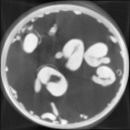
\includegraphics[width=\textwidth]{../images/sprouts/template_1.png}
\captionsetup{labelformat=empty}
        \caption{}
    \end{subfigure}
\quad
    \begin{subfigure}[b]{0.3\linewidth}
        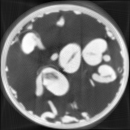
\includegraphics[width=\textwidth]{../images/sprouts/template_2.png}
\captionsetup{labelformat=empty}
        \caption{}
     \end{subfigure}
\quad
    \begin{subfigure}[b]{0.3\linewidth}
        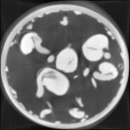
\includegraphics[width=\textwidth]{../images/sprouts/template_3.png}
\captionsetup{labelformat=empty}
        \caption{}
     \end{subfigure}\\
    \begin{subfigure}[b]{0.3\linewidth}
        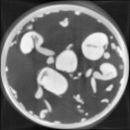
\includegraphics[width=\textwidth]{../images/sprouts/template_4.png}
\captionsetup{labelformat=empty}
        \caption{}
     \end{subfigure}
\quad
    \begin{subfigure}[b]{0.3\linewidth}
        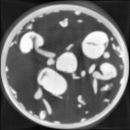
\includegraphics[width=\textwidth]{../images/sprouts/template_5.png}
\captionsetup{labelformat=empty}
        \caption{}
     \end{subfigure}
\quad
    \begin{subfigure}[b]{0.29\linewidth}
        \fcolorbox{white}{yellow}{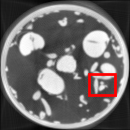
\includegraphics[width=\textwidth]{../images/sprouts/testIm_red.png}}
\captionsetup{labelformat=empty}
        \caption{}
     \end{subfigure}
      \caption{Sprouts 3D dataset: One slice each from the scanned
        objects that are used as templates (the first five from
        left) and a slice from the test (extreme right). One of the
        many regions in the test that is different from all other
        templates is the structure within the red box.}
\label{fig:object-prior_test_sprouts}
\addtolength{\textfloatsep}{-0.8cm}
\end{figure}

\textit{Remark:} In contrast to the scientific experiment performed
for the case of the okra and potato where we introduced man-made
defects, the changes in the sprouts here are purely the work of
nature. This dataset therefore has a different set of challenges.

%----------------------------------------Method-------------------------
\section{Spatially-Varying prior-based reconstruction}
\label{sec:method_spatially_varying_prior}
Our method modifies the algorithm presented in~\cite{my_dicta_paper}
and additionally overcomes one of its major limitations by introducing
an extra computational step. We first review the eigenspace-cum-CS
prior-based reconstruction algorithm which was
shown~\cite{my_dicta_paper} to be better when compared to
dictionary-based priors. PCA has been traditionally used
to find the significant modes of (Gaussian corrupted) data. In this
regard, it has been widely applied in the context of data
compression. However, PCA can also be seen as a tool to provide an
orthogonal basis to represent the space in which most of the test data
could lie (except the new changes). This space is constructed from the
available set of previously scanned objects which must cover a
realistically representative range of structures. %A preliminary version of this particular

To begin with,
when an object is scanned multiple times, a set of high quality
reconstructions (i.e., reconstructions from a dense set of
projection views) may be chosen as object-prior for the reconstruction
of future scan volumes, which in turn, may be scanned using far fewer
measurements. The eigenspace $E_{\text{high}}$ of the $L$ previously
scanned objects $Q_1,Q_2,...,Q_L$ is pre-computed. Here, it is assumed
that most of the test volume, barring the new changes, can be
expressed as a sparse linear combination of the principal components
(eigenvectors of the covariance matrix) obtained from a group of
structurally similar volumes. Hence, the object-prior is represented
by means of PCA. For the eigenspace to encompass a range of possible
structures in the test slice, the object-prior must represent a wide
structural range. Moreover, if these volumes are not aligned, then
they must be first registered before computing the prior.

The prior is built by computing the covariance matrix from the
template set $\{Q_i\}_{i=1}^L$. The space spanned by the eigenvectors
$\{\boldsymbol{V_p}\}_{p=1}^{L-1}$ (eigenspace) of the covariance
matrix is the object prior and is assumed to contain most of the test
slice (or volume in the case of 3D) that is similar, but not
necessarily identical to the object-prior. We use all of the $L-1$
orthogonal eigenvectors as a basis to represent the unknown test
volume. Let $\boldsymbol{\mu}$ denote the mean of the previously
scanned objects, and $\boldsymbol{\alpha}$ the unknown vector of
eigen-coefficients of the test scan, of which $\alpha_p$ is the
$p^{\textrm{th}}$ element. Then, once the eigenspace is pre-computed,
the test was reconstructed in~\cite{my_dicta_paper} by imposing a
penalty if the estimated slice does not lie within the eigen-space of
the object prior. Although such a prior can be very useful in some circumstances, it poses a limitation when we want accurate details of a portion of
the new changes. While the object prior compensates very well for the
possible artefacts due to sparse measurements, it may dominate the
regions with new changes masking the signal. \\

Ideally, we will want to
impose the prior only in the regions that are common between the test
and object-prior.  Our spatially-varying prior based reconstruction
overcomes this limitation by minimizing the following cost function:
\begin{equation}
  \begin{split}
%   \setlength{\belowdisplayskip}{0pt} \setlength{\belowdisplayshortskip}{0pt}
%\setlength{\abovedisplayskip}{-2pt} \setlength{\abovedisplayshortskip}{-2pt}
  J_3(\boldsymbol{x},\boldsymbol{\alpha}) = &\lVert\boldsymbol{\mathcal{R} x}-\boldsymbol{y}\rVert_2^2  + \lambda_1TV(\boldsymbol{x}) +\\
  &\lambda_2\lVert\boldsymbol{W}(\boldsymbol{x} - (\boldsymbol{\mu} + \sum_{p}\boldsymbol{V_p}\alpha_p))\rVert_2^2.
  \label{eq:spatially_varying_prior}
  \end{split}
\end{equation}


The key to our method is the discovery of a diagonal weights matrix
$\boldsymbol{W}$, where $W_{ii}$ contains the (non-negative) weight
assigned to the $i^{\textrm{th}}$ voxel of the prior. $\boldsymbol{W}$
is first constructed using some preliminary reconstruction methods,
following which Eq.~\ref{eq:spatially_varying_prior} is used to obtain
the final reconstruction. In regions of change in test data, we want
lower weights for the prior when compared to regions that are similar
to the prior.

$\lambda_1$ and $\lambda_2$ are tunable weights given to the TV-prior
and object-prior terms respectively and the specification of these are
discussed in Section.~\ref{sec:tuning_parameters}. The unknowns
$\boldsymbol{x}$ and $\boldsymbol{\alpha}$ are solved by alternately
minimizing $J_{\boldsymbol{\alpha}}(\boldsymbol{x})$ using a fixed
$\boldsymbol{\alpha}$, and $J_{\boldsymbol{x}}(\boldsymbol{\alpha})$
using the resultant $\boldsymbol{x}$.
$J_{\boldsymbol{\alpha}}(\boldsymbol{x})$ is solved for using an
optimal first-order method for large-scale TV regularization presented
in~\cite{TVReg} and available in~\cite{TVReg-lib}.

\begin{equation}
  \begin{split}
    J_{\boldsymbol{\alpha}}(\boldsymbol{\x}) \triangleq &\lVert\boldsymbol{\mathcal{R} x- y}\rVert_2^2  + \lambda_1TV(\boldsymbol{x}) \\
    &+\lambda_2\lVert(\boldsymbol{W}(\boldsymbol{x} - (\boldsymbol{\mu + V\alpha}))\rVert_2^2
  \end{split}
    \label{eq:compute_x}
  \end{equation}
  
\begin{equation}
  J_{\boldsymbol{x}}(\boldsymbol{\alpha}) \triangleq \lVert{\boldsymbol{W}(\boldsymbol{x}} - (\boldsymbol{\mu + V\alpha}))\rVert_2^2.
\end{equation}

Solving for $\boldsymbol{\alpha}$ leads to the closed form update:

\begin{equation}
  \boldsymbol{\alpha} = [(\boldsymbol{WV})^T\boldsymbol{WV}]^{-1}\boldsymbol{V}^T(\boldsymbol{W}^T\boldsymbol{W}(\boldsymbol{x} - \boldsymbol{\mu}))
  \label{eq:compute_alpha}
\end{equation}

%Optimal values of $\lambda_1, \lambda_2$ must be empirically chosen \textit{a priori}, based on the reconstructions of one of the template volumes (see also Sec.~\ref{sec:discussion}).
The cost function described in Eq.~\ref{eq:spatially_varying_prior} is biconvex and the convergence of this optimization is guaranteed by the monotone convergence theorem~\cite{monotone}.

\textbf{Computation of weights matrix $\boldsymbol{W}$:}
Since the test is unknown to
begin with, it is not possible to decipher the precise regions in
$\boldsymbol{x}$ that are different from all the previously scanned
objects (`object-prior'). We start with $X^{\text{fdk}}$, the initial
backprojection reconstruction of the test volume using FDK in an attempt to
discover the difference between the object-prior and the test
volume. Let $\boldsymbol{V_{\text{high}}}$ be the eigenspace
constructed from high-quality object-prior. However, the difference
between $X^{\text{fdk}}$ and its projection onto the eigenspace
$\boldsymbol{V_{\text{high}}}$ will detect the new regions along with
many false positives (false new regions). This is because,
$X^{\text{fdk}}$ will contain many geometric-specific artefacts
arising from sparse measurements (angle undersampling), which are
absent in the high quality object-prior used to construct the
eigenspace $\boldsymbol{V_{\text{high}}}$. To discover unwanted
artefacts of the imaging geometry, in a counter-intuitive way, we
generate \emph{low quality} reconstruction of the object-prior as
described below.  The algorithm is discussed next (a simplified version
appears as a schematic in the supplementary material and may be used
to understand the intuition.)

\textbf{Algorithm to compute weights-map $\boldsymbol{W}$:}
\label{sec:thealgo}
\begin{enumerate}

\item Perform a pilot reconstruction $X^{\text{fdk}}$ of the
  test volume $\boldsymbol{x}$ using FDK.

\item Compute low quality template volumes $Y^\text{fdk}$. 
We assume $L$ previously scanned objects from which we build
an eigenspace. 
\vspace{-0.1cm}

\begin{enumerate}
  \item Generate simulated measurements $\boldsymbol{y_{Q_i}}$ for
    every template $Q_i$, using the exact same projections views and
    imaging geometry with which the measurements $\boldsymbol{y}$ of
    the test volume $\boldsymbol{x}$ were acquired, and
\item Perform $L$ preliminary FDK reconstructions of each of the $L$
  object-prior from $\boldsymbol{y_{Q_i}}$.  Let this be denoted by
  $\{Y^{\text{fdk}}_i\}_{i=1}^L$.
  \end{enumerate}
\item Build eigenspace $\boldsymbol{V_{\text{low}}}$ from
  $\{Y^{\text{fdk}}_i\}_{i=1}^L$.  Let $P^{\text{fdk}}$ denote
  projection of $X^{\text{fdk}}$ onto
  $\boldsymbol{V_{\text{low}}}$. The difference between
  $P^{\text{fdk}}$ and $X^{\text{fdk}}$ will not contain false
  positives due to imaging geometry, but will have false positives due
  to artefacts that are specific to the reconstruction method used. To
  resolve this, perform steps $4$ and $5$.
%\vspace{-0.3cm}
\item Project with multiple methods.
%\vspace{-0.1cm}
  \begin{enumerate}
  \item Perform pilot reconstructions of the test using $M$ different
    reconstruction algorithms like the CS~\cite{lasso} with any
    suitable sparsity domain such as wavelets (Haar) or  DCT, Total
    Variation~\cite{TV}, Algebraic Reconstruction Technique
    (ART)~\cite{art}, Simultaneous Algebraic Reconstruction Technique
    (SART)~\cite{sart} and Simultaneous Iterative Reconstruction
    Technique (SIRT)~\cite{sirt}. Let this set of pilot
    reconstructions be denoted as $X \triangleq \{X^j\}_{j=1}^M$ where
    $j$ is an index for the reconstruction method, and $X^1 =
    X^{\text{fdk}}$.

  \item From $\boldsymbol{y_{Q_i}}$, perform reconstructions of the
    template $Q_i$ using the $M$ different algorithms, for each of the
    $L$ previously scanned objects. Let this set\footnote{If the set of projection views for every test is fixed a priori, this set of low quality reconstructions can be produced offline and stored, in order to save computational costs. If new sets of projection views for every test are to be allowed, the low quality reconstructions can still be performed efficiently using parallelization.} be denoted by $Y
    \triangleq \{\{Y_{i}^j\}_{j=1}^M\}_{i=1}^L$ where $Y^{1}_i =
    Y^{\text{fdk}}_i$, $\forall i \in \{1,..,,L\}$. 


  \item For each of the $M$ algorithms (indexed by $j$), build an
    eigenspace $\boldsymbol{V_\text{low}^j}$ from $\{Y_1^j,Y_2^j,
    \ldots, Y_{L}^j\}$. %($j=1..M$).

  \item Next, for each $j$, project $X^j$ onto
    $\boldsymbol{V_\text{low}^j}$. Let this projection be denoted by
    $P^j$. To reiterate, this captures those parts of the test volume
    that lie in the subspace $\boldsymbol{V_\text{low}^j}$ (i.e., are
    similar to the template reconstructions). The rest, i.e., new
    changes and their reconstruction method-dependent-artefacts, are
    not captured by this projection and need to be eliminated.
  \end{enumerate}
%\vspace{-0.1cm}
\item To remove all reconstruction method dependent false positives,
  we compute $\min_{j}(|X^j(x,y,z) - P^j(x,y,z)|)$. (The intuition for
  using the `min' is provided in the paragraph immediately following
  step 6 of this procedure.)
\item Finally, the weight to prior for each voxel coordinate $(x,y,z)$
  is given by
  \begin{equation} 
    \boldsymbol{W_v}(x,y,z) = (1+k(\min_{j}|X^j(x,y,z) - P^j(x,y,z)|))^{-1}.
    \label{eq:weightsEq}
  \end{equation}
\end{enumerate}
\vspace{0.01mm} Note that here $\boldsymbol{W_v}(x,y,z)$ represents
the weight to the prior in the $(x,y,z)^{th}$
voxel. $\boldsymbol{W_v}(x,y,z)$ must be low whenever the preliminary
test reconstruction $X^j(x,y,z)$ is different from its projection
$P^j(x,y,z)$ onto the prior eigenspace, for \emph{every} method $j \in
\{1,...,M\}$. This is because it is unlikely that \emph{every}
algorithm would produce a significant artefact at a voxel, and hence
we hypothesize that the large difference has arisen due to genuine
structural changes. This hypothesis is empirically and quantitatively
proven in the next section.  The parameter $k$ decides the sensitivity
of the weights to the difference $|X^j(x,y,z) - P^j(x,y,z)|$.
%It must be chosen empirically based on the reconstruction of one of the template
%volumes. 
Selection of $k$ is discussed in detail in Sec.~\ref{sec:discussion}.\\
%-------------------------------------------

%----------------------------------------Results-----------------------
\section{Results}
\label{sec:results_spatially_varying_prior}


In this section, we first illustrate the advantage of using multiple
types of eigenspaces for the computation of weights map, and then
present reconstruction results on all datasets.  We show both
qualitative and quantitative results.  Before we do this, it is import
to first consider our method of reporting our results.

\subsection{Metrics}
In order to show the efficacy, we will clearly need to have either a
gold-standard method, or a ground truth reference reconstruction such
as those described in Sec~\ref{sec:datasets} (see, for example, the
top left figure in Fig.~\ref{fig:story}).  For quantitative results,
we use two metrics: the Root Mean Squared Error (RMSE) and the
Structural Similarity Index Metric (SSIM)~\cite{ssim}.
% If
% $\boldsymbol{x}$ is the groundtruth data with $N$ voxels and
% $\hat{\boldsymbol{x}}$ is the reconstructed data, then RMSE is
% computed as follows

% \begin{equation}
%   \textrm{RMSE} =\sqrt{\frac{1}{N}\sum_{i=1}^N(\boldsymbol{x}(i) -
%     \hat{\boldsymbol{x}}(i))^2}.
%  \end{equation}
RMSE corresponds to error in intensity values and is a measure of
absolute error. Our results depend on the optimization library (as
mentioned earlier) \cite{TVReg-lib}; however, the range of values
returned by other libraries (such as the Matlab implementation of FDK
used in our ground truth reconstructions) are not compatible with
these.  This is not an issue for qualtitative results since the
display program compensates for range differences. For RMSE, and
for purposes of normalization and a fair comparison, while reporting
numbers, we therefore rescale intensity values of both the ground
truth and the reconstructed results to lie between 0 to 1, so that the
best possible RMSE is 0, and the worst value is 1.

On the other hand, SSIM seeks to consider perceptual changes, as well
as correlation between adjacent pixels. This can be useful in a
clinical context. The SSIM~\cite{multiscale_ssim} was designed to
flexible set coefficients for the following three factors: Structure,
Contrast and Intensity. We observed that in many cases, our
qualitative results (e.g., when the standard TV regularization method
outperforms FDK) do not correspond favourably to the default SSIM settings.  We
therefore assigned the following coefficients to the factors
Structure, Contrast, and Intensity respectively: $0.7,0.2,0.1$. Our
results are optimized for structure-focussed SSIM, but it can be
verified that in all cases for the various datasets considered, our
results are favourable with either the default metric, i.e, with
coefficients $1.0,1.0,1.0$ or with our structure-focused metric
wherein we assign a relatively higher weightage to structure
preservation.

%The reason for emphasizing the structure with an
%exponent of 0.7 stems from the optimization process since the
%intensity span (and, in general, the histogram) of reconstructed volumes
%differ across various methods and solvers. 

Finally, for a fair comparison in order to not distort metrics,
we report these values in what we believe is a reasonable area of
``new regions''. In particular, these regions of interest (RoI) are
obviously not known in advance, and is thus appropriate for a ``test''.


\subsection{Hyper-parameters}
\label{sec:tuning_parameters}

Next, we turn to the parameters of the algorithm.  $\lambda_1$,
$\lambda_2$ and $k$ are the three hyper-parameters that need to be
chosen carefully for best results. Since the aim of our experiments is
to demonstrate the benefit of using weighted prior reconstruction, we
proceed to adjust these parameters by (as mentioned earlier) assuming
the ground-truth to be known.

Specifically, $\lambda_1$ was tuned to maximize the SSIM of the
complete reconstructed test volume using the TV-only regularizer.
It's important to note that we retain this value of $\lambda_1$ for
the spatially-varying prior-based reconstruction, i.e., we \emph{do
  not} adjust this value for our spatially-varying method, and,
neither do we know the target ROI where the metric is going to be
finally employed.  With the already chosen optimal $\lambda_1$, we
apply our method for a range of $\lambda_2$ values and select the one
that gives the best SSIM with reference to the ground
truth. %The value of $\lambda_2$ influences the amount of artefacts that can be removed by the use of object-prior at the expense of its dominance in new regions. %This value was found to lie between $(0,3)$ for our datasets.
%In principle, one could have jointly optimized both $\lambda_1$ and
%$\lambda_2$ to get even better results compared to the one we have in
%Sections~\ref{sec:results_with_imaging_model},
%and~\ref{sec:results_without_imaging_model}.  
We note that in practice, however, since ground-truth will never be
available, these parameters must be tuned using only the set of
templates available.  One of the templates can be assumed to be a
pseudo-test, and a grid search can be performed to get the best
possible hyperparameter values. These values can then be used for
reconstructing the `real' test volume. 

%in the nvone may select $\lambda_2$ omnisciently only while imaging a
%particular class of object (say `sprouts') for the first time, and
%thereafter retain the same $\lambda_2$ while imaging other objects of
%the same class in future.  


$k$ defines the sensitivity of the weights map to
the difference between test image and object-prior (projection of test
onto the space of object-prior). When $k=0$, our method behaves
similar to the reconstruction using TV-only regularization. As $k$
increases, the weights map starts capturing new changes in the test,
at the cost of detecting a few false positives i.e., false new
changes. In other words, as the weights-map becomes more sensitive to
the difference between the test and object-prior, it becomes more
noisy. In order to visualize the effect of the hyper-parameter $k$, we
performed 2D reconstructions on okra dataset for different values of
$k$. Fig.~\ref{fig:few_view_okra_2D_weights} shows the weights map
obtained for each of the $k$ values and
Fig.~\ref{fig:reconstructions_as_k_varies} shows the corresponding
final reconstructions. We run our experiments for a few values of $k$
and empirically choose the best reconstruction based on our tolerance
for noise in the weights-map.  However, when a large number of
templates are available, instead of this empirical method, this
parameter can be chosen by assuming one of the templates as a
pseudo-test and validating the $k$ that results in the best
reconstruction (also see Sec~3 of \cite{supp_paper}).
%--------------effect of the value of $k$ on Okra dataset
\begin{figure}[h]
    \begin{subfigure}[b]{0.24\linewidth}
        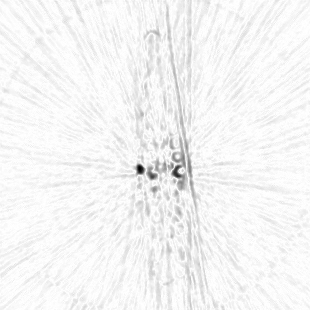
\includegraphics[width=\textwidth]{../images/okra/post_TCI/2D/48_views/tuning_k/weightsIm_kk_5_lambda_prior_0.700000.png}
        \caption{k=5}
     \end{subfigure}     
  \begin{subfigure}[b]{0.24\linewidth}
        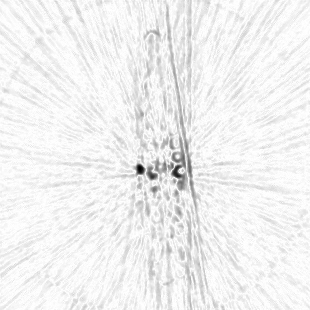
\includegraphics[width=\textwidth]{../images/okra/post_TCI/2D/48_views/tuning_k/weightsIm_kk_10_lambda_prior_0.700000.png}
        \caption{k=10}
     \end{subfigure} 
  \begin{subfigure}[b]{0.24\linewidth}
        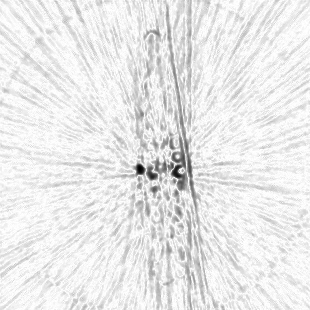
\includegraphics[width=\textwidth]{../images/okra/post_TCI/2D/48_views/tuning_k/weightsIm_kk_20_lambda_prior_0.700000.png}
        \caption{k=20}
     \end{subfigure}
  \begin{subfigure}[b]{0.24\linewidth}
        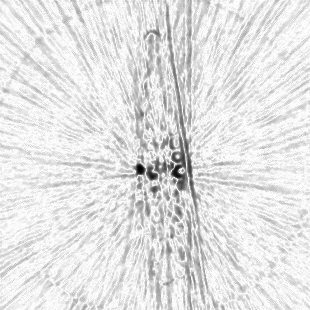
\includegraphics[width=\textwidth]{../images/okra/post_TCI/2D/48_views/tuning_k/weightsIm_kk_30_lambda_prior_0.700000.png}
        \caption{k=30}
     \end{subfigure}
  \begin{subfigure}[b]{0.24\linewidth}
        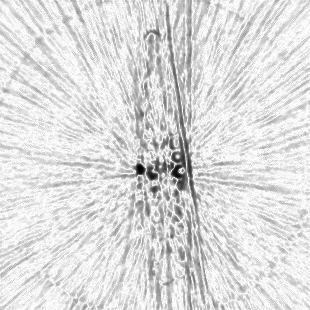
\includegraphics[width=\textwidth]{../images/okra/post_TCI/2D/48_views/tuning_k/weightsIm_kk_40_lambda_prior_0.700000.png}
        \caption{k=40}
     \end{subfigure}
  \begin{subfigure}[b]{0.24\linewidth}
        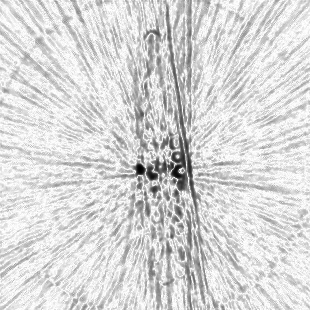
\includegraphics[width=\textwidth]{../images/okra/post_TCI/2D/48_views/tuning_k/weightsIm_kk_50_lambda_prior_0.700000.png}
        \caption{k=50}
     \end{subfigure}
   \begin{subfigure}[b]{0.24\linewidth}
        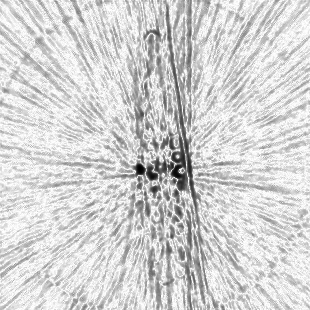
\includegraphics[width=\textwidth]{../images/okra/post_TCI/2D/48_views/tuning_k/weightsIm_kk_60_lambda_prior_0.700000.png}
        \caption{k=60}
     \end{subfigure}
   \begin{subfigure}[b]{0.24\linewidth}
        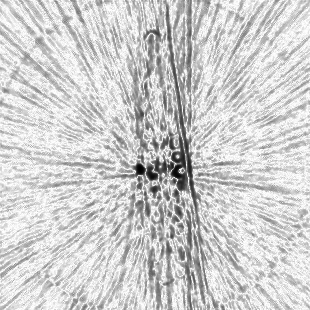
\includegraphics[width=\textwidth]{../images/okra/post_TCI/2D/48_views/tuning_k/weightsIm_kk_70_lambda_prior_0.700000.png}
        \caption{k=70}
     \end{subfigure}
  \begin{subfigure}[b]{0.24\linewidth}
        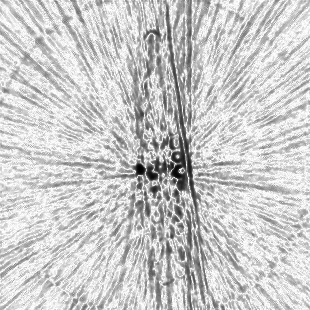
\includegraphics[width=\textwidth]{../images/okra/post_TCI/2D/48_views/tuning_k/weightsIm_kk_80_lambda_prior_0.700000.png}
        \caption{k=80}
     \end{subfigure}
   \begin{subfigure}[b]{0.24\linewidth}
        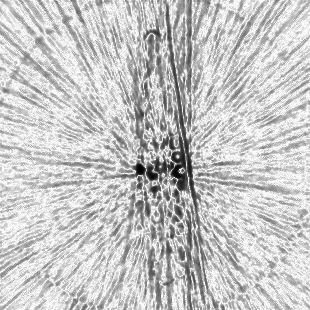
\includegraphics[width=\textwidth]{../images/okra/post_TCI/2D/48_views/tuning_k/weightsIm_kk_90_lambda_prior_0.700000.png}
        \caption{k=90}
     \end{subfigure}
   \begin{subfigure}[b]{0.24\linewidth}
        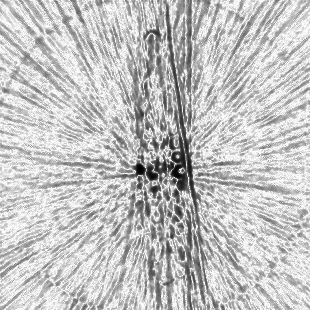
\includegraphics[width=\textwidth]{../images/okra/post_TCI/2D/48_views/tuning_k/weightsIm_kk_100_lambda_prior_0.700000.png}
        \caption{k=100}
     \end{subfigure}
   \begin{subfigure}[b]{0.24\linewidth}
        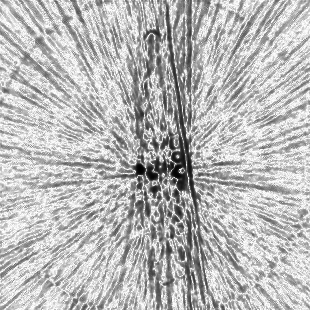
\includegraphics[width=\textwidth]{../images/okra/post_TCI/2D/48_views/tuning_k/weightsIm_kk_130_lambda_prior_0.700000.png}
        \caption{k=130}
     \end{subfigure}
    \caption{Different weights-maps for okra reconstruction. Low intensity denotes regions of new changes in test.}
\label{fig:few_view_okra_2D_weights}
\end{figure}
\begin{figure}[h]
    \begin{subfigure}[b]{0.24\linewidth}
        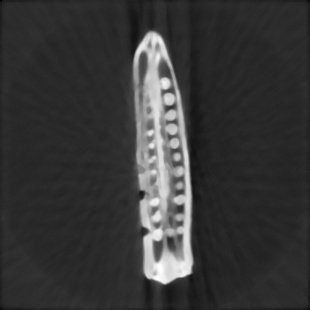
\includegraphics[width=\textwidth]{../images/okra/post_TCI/2D/48_views/tuning_k/weighted_prior_kk_5_lambda_prior_0.700000.png}
        \caption{k=5,\\ SSIM = 0.79}
     \end{subfigure}     
  \begin{subfigure}[b]{0.24\linewidth}
        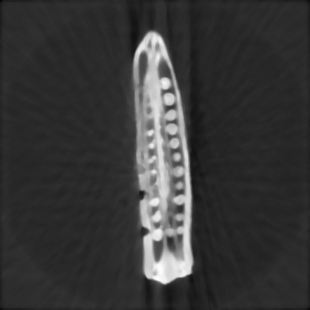
\includegraphics[width=\textwidth]{../images/okra/post_TCI/2D/48_views/tuning_k/weighted_prior_kk_10_lambda_prior_0.700000.png}
        \caption{k=10,\\ SSIM = 0.78}
     \end{subfigure} 
  \begin{subfigure}[b]{0.24\linewidth}
        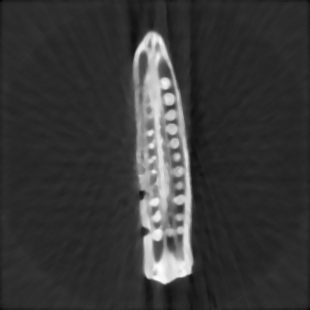
\includegraphics[width=\textwidth]{../images/okra/post_TCI/2D/48_views/tuning_k/weighted_prior_kk_20_lambda_prior_0.700000.png}
        \caption{k=20,\\ SSIM = 0.76}
     \end{subfigure}
  \begin{subfigure}[b]{0.24\linewidth}
        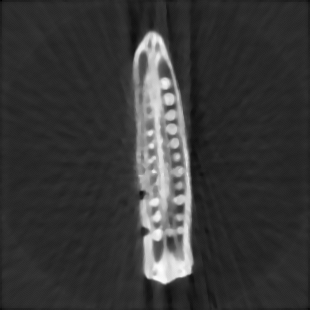
\includegraphics[width=\textwidth]{../images/okra/post_TCI/2D/48_views/tuning_k/weighted_prior_kk_30_lambda_prior_0.700000.png}
        \caption{k=30,\\ SSIM = 0.74}
     \end{subfigure}
  \begin{subfigure}[b]{0.24\linewidth}
        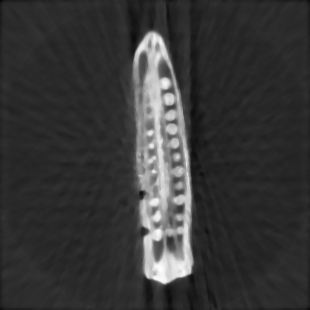
\includegraphics[width=\textwidth]{../images/okra/post_TCI/2D/48_views/tuning_k/weighted_prior_kk_40_lambda_prior_0.700000.png}
        \caption{k=40,\\ SSIM = 0.72}
     \end{subfigure}
  \begin{subfigure}[b]{0.24\linewidth}
        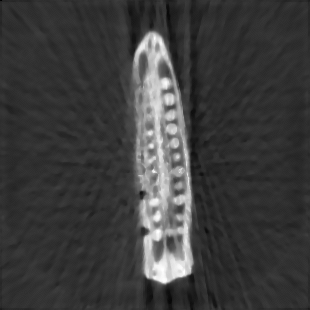
\includegraphics[width=\textwidth]{../images/okra/post_TCI/2D/48_views/tuning_k/weighted_prior_kk_50_lambda_prior_0.700000.png}
        \caption{k=50,\\ SSIM = 0.63}
     \end{subfigure}
   \begin{subfigure}[b]{0.24\linewidth}
        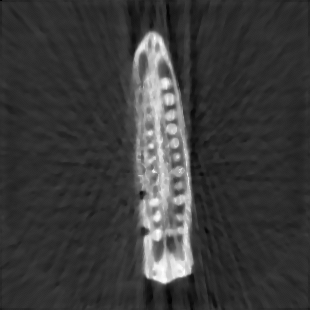
\includegraphics[width=\textwidth]{../images/okra/post_TCI/2D/48_views/tuning_k/weighted_prior_kk_60_lambda_prior_0.700000.png}
        \caption{k=60,\\ SSIM = 0.61}
     \end{subfigure}
   \begin{subfigure}[b]{0.24\linewidth}
        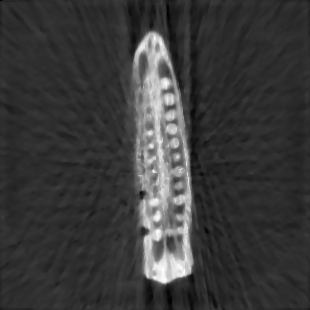
\includegraphics[width=\textwidth]{../images/okra/post_TCI/2D/48_views/tuning_k/weighted_prior_kk_70_lambda_prior_0.700000.png}
        \caption{k=70,\\ SSIM = 0.59}
     \end{subfigure}
  \begin{subfigure}[b]{0.24\linewidth}
        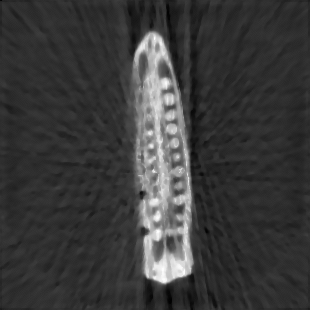
\includegraphics[width=\textwidth]{../images/okra/post_TCI/2D/48_views/tuning_k/weighted_prior_kk_80_lambda_prior_0.700000.png}
        \caption{k=80,\\ SSIM = 0.58}
     \end{subfigure}
   \begin{subfigure}[b]{0.24\linewidth}
        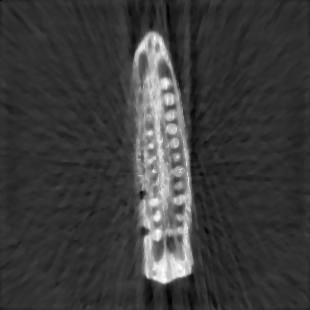
\includegraphics[width=\textwidth]{../images/okra/post_TCI/2D/48_views/tuning_k/weighted_prior_kk_90_lambda_prior_0.700000.png}
        \caption{k=90,\\ SSIM = 0.56}
     \end{subfigure}
   \begin{subfigure}[b]{0.24\linewidth}
        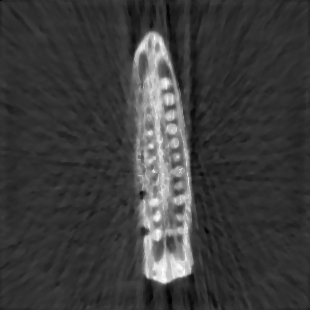
\includegraphics[width=\textwidth]{../images/okra/post_TCI/2D/48_views/tuning_k/weighted_prior_kk_100_lambda_prior_0.700000.png}
        \caption{k=100,\\ SSIM = 0.55}
     \end{subfigure}
   \begin{subfigure}[b]{0.24\linewidth}
        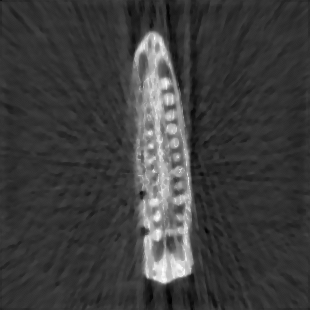
\includegraphics[width=\textwidth]{../images/okra/post_TCI/2D/48_views/tuning_k/weighted_prior_kk_130_lambda_prior_0.700000.png}
        \caption{k=130,\\ SSIM = 0.53}
     \end{subfigure}
    \caption{2D reconstructions for varying values of $k$. The SSIM (structure-focussed) values for all images are computed within the red RoI (shown in Fig.~\ref{fig:okra_2D_results}(a)), the region where the test is different from all of the previously scanned objects.}
\label{fig:reconstructions_as_k_varies}
\end{figure}

Our supplementary material~\cite{supp_paper} (part-3) discusses an alternate reconstruction method that does not require two of the three hyperparameters: $\lambda_1$ and $\lambda_2$. In this method, the computed weights-map is used to stitch parts of the pilot reconstruction and object-prior based on the weights map, and hence there is no optimization to be solved involving $\lambda_1$ and $\lambda_2$. The computation of weights map alone requires selection of the hyperparameter value k.


\subsection{Motivation for the use of multiple types of eigenspaces for the computation of weights}

The changes and new structures present in the test data will generate
different artifacts for different reconstruction techniques. These
artifacts would not be captured by reconstructions of the object-prior
since the underlying new changes and structures may be absent in all
of the previously scanned objects. We aim to let the weights be
independent of the type of artifact. Hence, we use a combination of
different reconstruction techniques to generate different types of
eigenspaces and combine information from all of them to compute the
weights map. To illustrate the benefit of this method, we first performed
2D reconstruction of a test slice from the potato dataset using
various reconstruction methods. We used implementations of algebraic
methods such as ART, SIRT and SART from~\cite{AIR_tools} and
implementations of CS solver from~\cite{l1ls}. Among various possible
sparsity basis for CS reconstruction, we observed that Haar wavelets
and DCT were best suited for this
dataset. Fig.~\ref{fig:potato_data_2D} shows the test and template
slices and Fig.~\ref{fig:weights_map_2Dpotato} shows the weights maps
generated using Eq.~\ref{eq:weightsEq} by various reconstruction
methods. It can be seen that the weights are low in the region of the
new change in test data. Because all the iterative methods are
computationally expensive, we chose only FBP and TV for computing
weights-maps for all 3D reconstructions.
%---------------------------------------


%-----------------------------potato data
\begin{figure}[!h]
    \begin{subfigure}[b]{0.24\linewidth}
        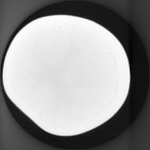
\includegraphics[width=\textwidth]{../images/potato/template_1.png}
%\captionsetup{labelformat=empty}       
 \caption{}
    \end{subfigure}
    \begin{subfigure}[b]{0.24\linewidth}
        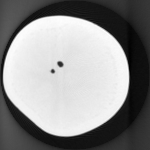
\includegraphics[width=\textwidth]{../images/potato/template_2.png}
%\captionsetup{labelformat=empty}
        \caption{}
     \end{subfigure}
    \begin{subfigure}[b]{0.24\linewidth}
        \includegraphics[width=\textwidth]{../images/potato/template_3.png}
%\captionsetup{labelformat=empty}
        \caption{}
     \end{subfigure}
    \begin{subfigure}[b]{0.235\linewidth}
        \fcolorbox{blue}{blue}{\includegraphics[width=\textwidth]{../images/potato/testIm_color.png}}
%\captionsetup{labelformat=empty}
        \caption{}
\label{fig:potato_test}
     \end{subfigure}
      \caption{Dataset for illustrating the use of multiple eigenspaces. (a)-(c): One slice each from the scanned objects, and (d): a slice from the test volume. Notice the appearance of the fourth hole in the test slice. }
\label{fig:potato_data_2D}
\end{figure}

%-----------------------------potato 2D weights
\begin{figure}[!h]
    \begin{subfigure}[b]{0.24\linewidth}
        \includegraphics[width=\textwidth]{../images/potato/post_tci/comparison/weightsIm_fbp30.png}
        \caption{FBP}
    \end{subfigure}
    \begin{subfigure}[b]{0.24\linewidth}
        \includegraphics[width=\textwidth]{../images/potato/post_tci/comparison/weightsIm_cs_dct30.png}
        \caption{CS-DCT}
     \end{subfigure}
    \begin{subfigure}[b]{0.24\linewidth}
        \includegraphics[width=\textwidth]{../images/potato/post_tci/comparison/weightsIm_cs_wavelet30.png}
        \caption{CS-Haar}
     \end{subfigure}
    \begin{subfigure}[b]{0.24\linewidth}
        \includegraphics[width=\textwidth]{../images/potato/post_tci/comparison/weightsIm_art30.png}
        \caption{ART}
     \end{subfigure}
    \begin{subfigure}[b]{0.24\linewidth}
        \includegraphics[width=\textwidth]{../images/potato/post_tci/comparison/weightsIm_sart30.png}
        \caption{SART}
     \end{subfigure}
    \begin{subfigure}[b]{0.24\linewidth}
        \includegraphics[width=\textwidth]{../images/potato/post_tci/comparison/weightsIm_sirt30.png}
        \caption{SIRT}
    \end{subfigure}
        \begin{subfigure}[b]{0.24\linewidth}
        \includegraphics[width=\textwidth]{../images/potato/post_tci/comparison/weightsIm_tv30.png}
        \caption{TV}
     \end{subfigure}
    \begin{subfigure}[b]{0.24\linewidth}
        \includegraphics[width=\textwidth]{../images/potato/post_tci/comparison/weightsIm_all_methods30.png}
        \caption{This paper}
     \end{subfigure}
      \caption{The motivation for multiple methods is demonstrated
        with a slice of the data in Fig.~\ref{fig:potato_data_2D}.
        The test image in Fig.~\ref{fig:potato_data_2D}(d) is
        reconstructed using only $6$ views.  The weights-maps
        %(corresponding to the difference between pilot reconstruction
        %of the test and its projection onto the eigenspace
        %$\boldsymbol{V_\text{low}}$) 
        constructed using different
        reconstruction methods individually (a)-(g) are inadequate and
        represent different false positives. By fusing information
        from all reconstruction methods, as specified in
        Eq.~\ref{eq:weightsEq} we get the final weights map (h). The corresponding reconstructions appear in Fig.~\ref{fig:reconstructions_diff_methods}}.
%The weights-maps are different because the reconstruction artefacts of the new structures in test image will be different for every reconstruction method used, as seen in Fig.~\ref{fig:reconstructions_diff_methods}. }
\label{fig:weights_map_2Dpotato}
\end{figure}
%-----------------------------potato 2D weights
\begin{figure}[!h]
    \begin{subfigure}[b]{0.24\linewidth}
        \includegraphics[width=\textwidth]{../images/potato/post_tci/comparison/fbp.png}
        \caption{FBP}
    \end{subfigure}
    \begin{subfigure}[b]{0.24\linewidth}
        \includegraphics[width=\textwidth]{../images/potato/post_tci/comparison/cs_dct.png}
        \caption{CS-DCT}
     \end{subfigure}
    \begin{subfigure}[b]{0.24\linewidth}
        \includegraphics[width=\textwidth]{../images/potato/post_tci/comparison/cs_wavelet.png}
        \caption{CS-Haar}
     \end{subfigure}
    \begin{subfigure}[b]{0.24\linewidth}
        \includegraphics[width=\textwidth]{../images/potato/post_tci/comparison/art.png}
        \caption{ART}
     \end{subfigure}
    \begin{subfigure}[b]{0.24\linewidth}
        \includegraphics[width=\textwidth]{../images/potato/post_tci/comparison/sart.png}
        \caption{SART}
     \end{subfigure}
    \begin{subfigure}[b]{0.24\linewidth}
        \includegraphics[width=\textwidth]{../images/potato/post_tci/comparison/sirt.png}
        \caption{SIRT}
    \end{subfigure}
        \begin{subfigure}[b]{0.24\linewidth}
        \includegraphics[width=\textwidth]{../images/potato/post_tci/comparison/tv.png}
        \caption{TV}
     \end{subfigure}
    \begin{subfigure}[b]{0.24\linewidth}
        \includegraphics[width=\textwidth]{../images/potato/post_tci/comparison/weighted_pca_all_methods30.png}
        \caption{This paper}
     \end{subfigure}
      \caption{(a)-(g): Reconstructions of~\ref{fig:potato_data_2D}(d)
        from $6$ views. The magnitude and sharpness of the artefacts
        are different for distinct methods. (h)
        Spatially-Varying-prior method (from this paper) combines
        weights-map information from all other methods. Quantitative
        metrics for evaluation  of
        these reconstructions are shown in
        Table.~\ref{table:potato_2D_ssim}.}
\label{fig:reconstructions_diff_methods}
\end{figure}
%----------------------------------------------
\begin{table}[!h]
  \centering
\caption{Default-SSIM (`SSIM-1'), structure-focussed SSIM (`SSIM-2') and RMSE of the reconstructions shown in
  Fig.~\ref{fig:reconstructions_diff_methods}:(a)-(h). %The SSIM of
                                %ideal reconstruction is 1. The ideal
                                %RMSE is 0, and the worst RMSE
                                %possible is 1 here.
}
\begin{tabular}{|l|c|c|c|c|c|c|c|c|c|}
\hline
& \textbf{(a)} & \textbf{(b)} & \textbf{(c)} & \textbf{(d)} & \textbf{(e)} & \textbf{(f)} &  \textbf{(g)} &  \textbf{(h)} \\\hline
SSIM-1 & 0.31 & 0.48  & 0.39  & 0.51 & 0.55  & 0.42 & 0.68 &\textcolor{red}{0.78} \\ \hline
SSIM-2 & 0.64 & 0.72  & 0.68 & 0.83 & 0.81 & 0.69 & 0.83 &\textcolor{red}{0.88} \\ \hline
RMSE & 0.38 & 0.18 & 0.25 & 0.43 & 0.33 & 0.21 & 0.11 & \textcolor{red}{0.04}\\ \hline
\end{tabular}
\label{table:potato_2D_ssim}
\end{table}

\subsection{Reconstruction of datasets with imaging model available}
\label{sec:results_with_imaging_model}
\subsubsection{\textbf{Potato}}
\label{Sec:potato_spatially_varying}

The test volume was reconstructed from a partial set of $2\%$ of projection views from
which ground truth was reconstructed (see remarks in
Sec.~\ref{sec:potatoAndOkra}). 2D reconstructions of one of the slices
is shown in Fig.~\ref{fig:potato_2D_results}. A complete 3D
reconstruction can be found in the supplementary
material~\cite{supp_paper}. The red RoI spans 7 consecutive slices
where the test is different from all of the previously scanned
objects. %The zoomed-in images around the major region of change (red
%RoI) is shown in Fig.~\ref{fig:potato_zoomed_2D_results}. 
\begin{figure}[!h]
\centering
\subcaptionbox{Test}{\fcolorbox{blue}{blue}{\includegraphics[width=0.22\columnwidth]{../images/potato/post_tci/testIm_paper.png}}}
\subcaptionbox{FBP, no prior}{\includegraphics[width=0.23\columnwidth]{../images/potato/post_tci/6_views/fbp.png}}
\subcaptionbox{TV, no prior}{\includegraphics[width=0.23\columnwidth]{../images/potato/post_tci/6_views/tv_lambdaTV_0.05.png}}
\subcaptionbox{This paper}{\includegraphics[width=0.23\columnwidth]{../images/potato/post_tci/6_views/weighted_prior_kk_30_lambda_prior_1.100000.png}}
\caption{Reconstruction of potato from 6 projection views--(b) has strong streak artefacts with unclear structure of the potato, (c) largely blurred, and (c) is sharper with significantly reduced streak artefacts.}
\label{fig:potato_2D_results}
\end{figure}

We observe
that our method reconstructs new structures while simultaneously
reducing streak artefacts. Table~\ref{table:potato_ssim} shows SSIM and RMSE of
the reconstructed new regions using various methods. 
%The ground truth and reconstructions are normalized to lie in [0-1].
\begin{comment}
\begin{figure}[!h]
\centering
\subcaptionbox{Test}{\fcolorbox{blue}{blue}{\includegraphics[width=0.22\columnwidth]{../images/potato/post_tci/6_views/test_zoomed.png}}}
\subcaptionbox{FDK, no prior}{\includegraphics[width=0.23\columnwidth]{../images/potato/post_tci/6_views/fbp_zoomed.png}}
\subcaptionbox{TV, no prior}{\includegraphics[width=0.23\columnwidth]{../images/potato/post_tci/6_views/tv_zoomed.png}}
\subcaptionbox{This paper}{\includegraphics[width=0.23\columnwidth]{../images/potato/post_tci/6_views/weighted_pca_zoomed.png}}
\caption{A zoomed-in version of the regions around the RoI of the reconstructions shown in Fig.~\ref{fig:potato_2D_results}.}
\label{fig:potato_zoomed_2D_results}
\end{figure}
\end{comment}
%-------------------------------------------------------------------------
\begin{table}[!h]
  \centering
  \caption{Default-SSIM, structure-focussed SSIM and RMSE within the RoI of reconstructed potato from various
    methods. 
%The SSIM of ideal reconstruction is 1. The ideal RMSE is 0, and the worst RMSE possible is 1 here. 
The 2D reconstructed images are shown in Fig.~\ref{fig:potato_2D_results}, and 3D reconstructed volumes can be seen in~\cite{supp_paper}.}
\begin{tabular}{|l|c|c|c|c|c|}
\hline &
\textbf{Backprojection} & \textbf{TV} &
\textbf{This paper} \\ \hline \textbf{2D} & 0.22, 0.52, 0.36
& 0.86, 0.92, 0.06 & \textcolor{red}{0.95, 0.97, 0.03} \\ \hline \textbf{3D} & 0.30, 0.58, 0.26 & 0.56, 0.75, 0.21 & \textcolor{red}{0.72, 0.84, 0.16}
\\ \hline
\end{tabular}
\label{table:potato_ssim}
\end{table}

%--------------------------Okra-- results
\subsubsection{\textbf{Okra}}
\label{Sec:okra_spatially_varying}
The test volume was reconstructed from a partial set of $10\%$ of projection views from which
ground truth was reconstructed (refer Sec.~\ref{sec:datasets}). 2D reconstructions of one of the
slices is shown in Fig.~\ref{fig:okra_2D_results}. A complete 3D
reconstruction can be found in in the supplementary material
~\cite{supp_paper}. The red RoI spans 7 consecutive slices where the
test is different from all of the previously scanned objects. %A
%zoomed-in region around the major region of change (red RoI) is shown
%in Fig.~\ref{fig:okra_zoomed_2D_results}.
As in the test, the
reconstruction by spatially-varying method shows the absence of the
deformity and better removal of sub-sampling artefacts when compared
to FDK and TV. This is also seen in the SSIM and RMSE values in
Table~\ref{table:okra_ssim}. 
%The ground truth and reconstructions are normalized to lie in [0-1].


\begin{figure}[!h]
\centering
\subcaptionbox{Test}{\fcolorbox{cyan}{cyan}{\includegraphics[width=0.23\columnwidth]{../images/okra/post_TCI/2D/48_views/input_roi.png}}}
\subcaptionbox{FBP, no prior}{\includegraphics[width=0.23\columnwidth]{../images/okra/post_TCI/2D/48_views/FBP_cropped.png}}
\subcaptionbox{TV, no prior}{\includegraphics[width=0.23\columnwidth]{../images/okra/post_TCI/2D/48_views/TV_cropped.png}}
%\subcaptionbox{\mbox{Uniform}\\prior}{\includegraphics[width=0.19\columnwidth]{../images/okra/pca_cropped.png}}\hfill
\subcaptionbox{This paper}{\includegraphics[width=0.23\columnwidth]{../images/okra/post_TCI/2D/48_views/weighted_prior_cropped.png}}
\caption{Reconstruction of okra from 48 projection views
   (b) has streaky artefacts, (c) has blurred structures and (d) is sharper with significantly less streaky artefacts.}
\label{fig:okra_2D_results}
\end{figure}

\begin{comment}
\begin{figure}[!h]
\centering
\subcaptionbox{Test}{\fcolorbox{cyan}{cyan}{\includegraphics[width=0.22\columnwidth]{../images/okra/post_TCI/2D/48_views/test_zoomed.png}}}
\subcaptionbox{FDK, no prior}{\includegraphics[width=0.23\columnwidth]{../images/okra/post_TCI/2D/48_views/fbp_zoomed.png}}
\subcaptionbox{TV, no prior}{\includegraphics[width=0.23\columnwidth]{../images/okra/post_TCI/2D/48_views/tv_zoomed.png}}
%\subcaptionbox{\mbox{Uniform}\\prior}{\includegraphics[width=0.19\columnwidth]{../images/okra/pca_cropped.png}}\hfill
\subcaptionbox{This paper}{\includegraphics[width=0.23\columnwidth]{../images/okra/post_TCI/2D/48_views/weighted_pca_zoomed.png}}
\caption{A zoomed-in version of the regions around the RoI of the reconstructions shown in Fig.~\ref{fig:okra_2D_results}. }
\label{fig:okra_zoomed_2D_results}
\end{figure}
\end{comment}

%---------------------------------------
\begin{table}[!h]
  \centering
  \caption{Default-SSIM, structure-focussed SSIM and RMSE within the RoI of reconstructed okra from various
    methods. 
%SSIM of the ideal reconstruction is 1. The ideal RMSE is 0, and the worst RMSE possible is 1 here.  
The 2D reconstructed images are shown in Fig.~\ref{fig:okra_2D_results}, and 3D reconstructed volumes can be seen in~\cite{supp_paper}.}
\begin{tabular}{|l|c|c|c|c|c|}
\hline &
\textbf{Backprojection} & \textbf{TV} &
\textbf{This paper} \\ \hline \textbf{2D} & 0.26, 0.46, 0.28
& 0.27, 0.50, 0.24 & \textcolor{red}{0.56, 0.74, 0.15} \\ 
\hline \textbf{3D} & 0.52, 0.65, 0.22 & 0.56, 0.70, 0.21 & \textcolor{red}{0.57, 0.71, 0.19}
\\ \hline
\end{tabular}
\label{table:okra_ssim}
\end{table}

\subsection{Reconstruction of datasets without imaging model}
\label{sec:results_without_imaging_model}
\subsubsection{\textbf{Liver}}
\label{sec:tmh}

Here we show how our technique is useful in a
real-life medical longitudinal study. Our data consists of
successive scans of the liver taken during a radio-frequency ablation
procedure as described in Sec.~\ref{sec:datasets}. Our goal is to to
track the position of the needle in a relatively stationary
background, while simultaneously reducing sub-sampling artefacts.
Specifically, we choose slices 1-6 as our object-prior, and
reconstruct slice 7 from few-views with the specific goal of tracking
the needle and simultaneously reducing
artefacts. Fig.~\ref{fig:tmh_2D_results} 
shows reconstruction of the test
slice from its measurements from only 30 views. 
The ground truth and reconstructions 
%are normalized to lie in [0-1] and 
are quantitatively compared using
SSIM and RMSE in Table~\ref{table:tmh_ssim}.

%--------------------RFA 2 few views
\begin{figure}[!h]
\centering
\subcaptionbox{Test}{\fcolorbox{white}{green}{\includegraphics[width=0.23\columnwidth]{../images/tmh/RFA2/post_TCI/very_few_views/colorTestIm.png}}}\hfill
\subcaptionbox{FBP, no prior}{\includegraphics[width=0.24\columnwidth]{../images/tmh/RFA2/post_TCI/very_few_views/fbp.png}}\hfill
\subcaptionbox{TV, no prior}{\includegraphics[width=0.24\columnwidth]{../images/tmh/RFA2/post_TCI/very_few_views/tv_lambdaTV_0.036.png}}\hfill
\subcaptionbox{This paper}{\includegraphics[width=0.24\columnwidth]{../images/tmh/RFA2/post_TCI/very_few_views/weighted_prior_kk_30_lambda_prior_1.100000.png}}
\caption{\small{ Reconstruction of `test' (slice 7) from Fig.~\ref{fig:RFA2_test_object-prior} from only 30 views, using (b) FBP and no prior resulting in streaks (c) TV resulting in blurred bone structures and (d) spatially varying object-prior (slices 1-6 of Fig.~\ref{fig:RFA2_test_object-prior} are used as object-prior) resulting in clear bone structures with less streaks. The region enclosed in red rectangle is our Region of Interest (RoI) as it contains both the new position of the needle and some background.}}
\label{fig:tmh_2D_results}
\end{figure}

%\subcaptionbox{Weights map}{\includegraphics[width=0.24\columnwidth]{../images/tmh/RFA2/post_TCI/very_few_views/weightsIm_kk_30_lambda_prior_1.100000.png}}
\begin{comment}
\begin{figure}[!h]
\centering
\subcaptionbox{Test}{\fcolorbox{white}{green}{\includegraphics[width=0.23\columnwidth]{../images/tmh/RFA2/post_TCI/very_few_views/test_zoomed.png}}}\hfill
\subcaptionbox{Backprojection\\no prior}{\includegraphics[width=0.24\columnwidth]{../images/tmh/RFA2/post_TCI/very_few_views/fbp_zoomed.png}}\hfill
\subcaptionbox{TV, no prior}{\includegraphics[width=0.24\columnwidth]{../images/tmh/RFA2/post_TCI/very_few_views/tv_zoomed.png}}\hfill
\subcaptionbox{This paper}{\includegraphics[width=0.24\columnwidth]{../images/tmh/RFA2/post_TCI/very_few_views/weighted_pca_zoomed.png}}
\caption{A zoomed-in version of the regions around the RoI of the reconstructions shown in Fig.~\ref{fig:tmh_2D_results}.}
\label{fig:tmh_2D_zoomed_results}
\end{figure}
\end{comment}

\begin{table}[!h]
  \centering
  \caption{Default-SSIM, structure-focussed SSIM and RMSE within the RoI of 2D reconstruction of radio-frequency ablation data of liver from various methods.  
%For ideal reconstruction, SSIM equals 1. The ideal RMSE is 0, and the worst RMSE possible is 1 here.  
The  reconstructed images are shown in Fig.~\ref{fig:tmh_2D_results},}
\begin{tabular}{|l|c|c|c|c|}
\hline \textbf{Backprojection} & \textbf{TV} &
\textbf{This paper} \\ \hline 0.54, 0.73, 0.04
& 0.80, 0.91, 0.09 & \textcolor{red}{0.90, 0.95, 0.03} \\ \hline 
\end{tabular}
\label{table:tmh_ssim}
\end{table}
%-----------------------------------------------------------------



\subsubsection{\textbf{Sprouts}}
\label{Sec:sprouts_spatially_varying}
 %-----------------------------sprouts 3D results

The test volume was reconstructed from a partial set of  
 $1.7\%$ of projection views
from which ground truth was reconstructed (refer
Sec.~\ref{sec:datasets}). The selected 3D ground truth of template
volumes, test volume, as well as the 3D reconstructions are shown in
the supplementary material~\cite{supp_paper}. For the sake of
exposition, the red region of interest (RoI) has been culled out from
7 consecutive slices in the 3D volume to indicate new structures;
other changes can be viewed in the video.  2D reconstruction of one of
the slices is shown in Fig.~\ref{fig:sprouts_2D_results}.
Table~\ref{table:sprouts_ssim} shows the improvement in SSIM and RMSE of the
reconstructed new regions as compared to other methods. 
%The ground truth and reconstructions are normalized to lie in [0-1].
%----------------------------------------------------

\begin{figure}[!h]
\centering
\subcaptionbox{Test}{\fcolorbox{yellow}{yellow}{\includegraphics[width=0.22\columnwidth]{../images/sprouts/post_TCI/2D/20_views/testIm_roi.png}}}
\subcaptionbox{FBP, no prior}{\includegraphics[width=0.23\columnwidth]{../images/sprouts/post_TCI/2D/20_views/fbp.png}}
\subcaptionbox{TV, no prior}{\includegraphics[width=0.23\columnwidth]{../images/sprouts/post_TCI/2D/20_views/tv_lambdaTV_0.100.png}}
\subcaptionbox{This paper}{\includegraphics[width=0.23\columnwidth]{../images/sprouts/post_TCI/2D/20_views/weighted_prior_kk_30_lambda_prior_2.100000.png}}
\caption{Reconstruction of sprouts from 20 projection views
   (b) has streaky artefacts, (c) has blurred structures and (d) is sharper with significantly less streaky artefacts.}
\label{fig:sprouts_2D_results}
\end{figure}

%----------------------------------------------------
\begin{comment}
\begin{figure}[!h]
\centering
\subcaptionbox{Test}{\fcolorbox{yellow}{yellow}{\includegraphics[width=0.22\columnwidth]{../images/sprouts/post_TCI/2D/20_views/test_zoomed.png}}}
\subcaptionbox{FDK, no prior}{\includegraphics[width=0.23\columnwidth]{../images/sprouts/post_TCI/2D/20_views/fbp_zoomed.png}}
\subcaptionbox{TV, no prior}{\includegraphics[width=0.23\columnwidth]{../images/sprouts/post_TCI/2D/20_views/tv_zoomed.png}}
%\subcaptionbox{\mbox{Uniform}\\prior}{\includegraphics[width=0.19\columnwidth]{../images/okra/pca_cropped.png}}\hfill
\subcaptionbox{This paper}{\includegraphics[width=0.23\columnwidth]{../images/sprouts/post_TCI/2D/20_views/weighted_pca_zoomed.png}}
\caption{A zoomed-in version of the regions around the RoI of the reconstructions shown in Fig.~\ref{fig:sprouts_2D_results}}
\label{fig:sprouts_zoomed_2D_results}
\end{figure}
\end{comment}
%--------------------------------------------------------------
\begin{table}[!h]
  \centering
  \caption{Default-SSIM, structure-focussed SSIM and RMSE within the RoI of reconstructed sprouts from various
    methods. 
%The SSIM of ideal reconstruction) is 1. The ideal RMSE is 0, and the worst RMSE possible is 1 here. 
The 2D reconstructed images are shown in Fig.~\ref{fig:sprouts_2D_results}, and 3D reconstructed volumes can be seen in~\cite{supp_paper}.}
\begin{tabular}{|l|c|c|c|c|c|}
\hline &
\textbf{Backprojection} & \textbf{TV} & \textbf{This paper}
 \\ \hline \textbf{2D} & 0.42, 0.67, 0.24
& 0.61, 0.82, 0.17 & \textcolor{red}{0.72, 0.86, 0.13} \\ \hline \textbf{3D} & 0.44, 0.67, 0.25 & 0.47, 0.73, 0.23 & \textcolor{red}{0.66, 0.82, 0.14}
\\ \hline
\end{tabular}
\label{table:sprouts_ssim}
\end{table}

%--------------------------------------------------------------------------

%---------------------------------------------------------

\section{Computational Complexity}
\label{sec:discussion}
%In this section, we discuss computational
%complexity of our method and requirements for applying deep learning
%techniques in longitudinal few-view reconstruction.
%\subsection{Computational Complexity}

We discuss the computing burden of our method in two parts: the big-Oh
(symbolic) complexity, and the actual time taken on a specific dataset
on a specific computer. In the latter case, we provide the actual
code~\cite{codeRepo} for the purposes of reproduction. 

\subsubsection{Symbolic}
Let
\begin{itemize}
\item $N$ denote the number of voxels of test volume,
\item $L$ denote the number of templates available,
\item $M$ denote the number of pilot reconstruction algorithms used for the computation of weights map, and
\item $F$ denote the time taken for optimization.
  $F$ consists of time taken for alternate minimization of Eq.~\ref{eq:spatially_varying_prior}, which in turn consists of time taken for repeated cycles of a closed-form update of $\boldsymbol{\alpha}$ (Eq.~\ref{eq:compute_alpha}) and an iterative optimization of  $\boldsymbol{x}$ (Eq.~\ref{eq:compute_x}). 
\end{itemize}
We note that in practice $L$ is independent of $N$ and is likely to be
$O(1)$ (e.g., about 12 scans in a year for disease prognosis).
Likewise $M$ is also $O(1)$. The speed of the iterative optimization
is dependent on the number of imaging views, and is profoundly
impacted by the actual numerical optimization technique used.
Therefore, the time computational complexity of our method is sum of
the following
\begin{enumerate}
\item $O(NL^2+L^3)$ for creating eigenspaces, which is, in practice linear, i.e., $O(N)$.
\item $O(NLM)$ for deriving weights map, which is, in practice linear, i.e., $O(N)$.
\item and the time $F$  taken for iterative minimization, which as mentioned above is not the key contribution of this paper. 
\end{enumerate}
In short, the additional burden of the key idea of this paper viz.,
generating weights map is linear in the number of voxels, although
admittedly the burden $F$ of the alternate minimization procedure
drives up the cost (as can be seen in
Table~\ref{table:compute_time}). The supplementary material describes
a method to avoid this cost if absolutely necessary.

In terms of space, the complexity is $O(NL +N)$ to store each of the
$L$ templates and their low quality reconstructions, and to store one
weights map. We only need to store a single weights map volume
regardless of the number of templates available.

\subsubsection{Example Computation}
If the set of projection views for every test is fixed a priori, a
reasonable assumption, the set of low quality reconstructions can be
produced offline and stored in order to save computational costs. 
% Most of the computation time in our technique is used for the
% generation of low quality eigen-space by reconstructing each of the
% templates using TV and FDK. 
With this as the basis, Table~\ref{table:compute_time} shows the
computation times for various stages of reconstruction of a 2D slice
of Liver on MATLAB 2019a on an AMD
2920X 12-Core Processor machine with 64GB RAM. 
% If however, new sets of
% projection views for every test are to be allowed, the low quality
% reconstructions can still be performed efficiently using
% parallelization since these reconstructions are completely
% independent. 
\begin{table}[!h]
 \centering
  \caption{Computation times (in seconds) for various stages of
    reconstruction of a (512$\times$512) 2D slice of Liver from 30 views, on MATLAB 2019a on an  AMD
    2920X 12-Core Processor machine with 64GB RAM. Our code is
    available for inspection~\cite{codeRepo}.}
\begin{tabular}{|l|l|l|l|}
\hline
 \begin{tabular}[c]{@{}l@{}} FBP \end{tabular}             & \begin{tabular}[c]{@{}l@{}} TV  \end{tabular}                      & \begin{tabular}[c]{@{}l@{}}Computation of \\ weights map \end{tabular} & \begin{tabular}[c]{@{}l@{}}Alternate\\ Minimization \end{tabular} \\ \hline
\multicolumn{1}{|c|}{0.01} & \multicolumn{1}{c|}{5.63} & \multicolumn{1}{c|}{0.01}                                             & \multicolumn{1}{c|}{34.00}                                                                     \\ \hline
\end{tabular}
\label{table:compute_time}
\end{table}
\begin{comment}
\subsection{Requirements for applying deep learning techniques}
Deep learning techniques are powerful tools to learn an unknown
parametric function relating an input space and an output space. In such
settings, our current goal of detecting new changes is a `prediction'
problem in a continuous solution space i.e., \textit{``given
  intensities of a voxel at various time instants in a longitudinal
  setting and partial measurements of the voxel at the current time,
  what will be the intensity of the same voxel at the current time
  instant?''}. This estimation can be learned by a deep neural network
if there are hundreds of labeled data.  However, generalization of
this across multiple datasets poses a question mark.

  Further, a specific `event-of-interest' may occur just once in a
  longitudinal study and hence training on data from all previous time
  instants of the same specimen may be misleading. As a future work, measurements from
  identical and full-cycle longitudinal studies, including
  events-of-interest, from an \textit{atlas of similar specimen} can be used to train
  a deep learning model.  We  see this as an extension of using object-prior generated from the
  \textit{same specimen}.

  Another avenue for using deep networks \textit{within} our current
  work is to replace the currently used fixed eigenspace provided by
  PCA by a learned feature basis provided by a network such as an
  autoencoder. For each dataset, an autoencoder may be trained to
  learn a specific set of latent features. This will again require
  atleast a few tens of volumes. We see this as a future direction of
  work.
\end{comment}


%--------------------------Conclusion-----------------------
\section{Conclusions}
\label{sec:conclusions}
This work deals with the effective use of priors for tomographic
reconstruction in longitudinal studies. When the number of measurements 
impedes the benefit of applying classic regularization methods, we discuss the utility of
using information from previous scans of the same object, as outlined in
Figs.~\ref{fig:story} and~\ref{fig:prior_overview}. In order to observe details of new changes
accurately, we use a novel
spatially-varying prior-based method. This method ensures that the
reconstruction of localized new information in the data is not
affected by the priors, while the other relatively stationary regions benefit from the extra prior information. %Based on the potato and the okra experiments,
%we see that our method is able to \emph{discover both} the presence of
%a new structure, as well as the absence of a structure.
We have thus
improved state of the art by detecting the strength and location
of these regions of change and
assigning low prior weights wherever necessary. This innovation becomes evident through the weights maps shown in Figure~\ref{fig:weights_map_2Dpotato} and the resulting reconstructions shown in Figure~\ref{fig:reconstructions_diff_methods}. The probability of
presence of a `new region' is enhanced considerably by a novel
combination of different reconstruction techniques.  We have validated
our technique on medical 2D and real, biological 3D datasets for
longitudinal studies. The method is also largely robust to the number
of previously scanned objects used. We urge the reader to see the
videos of reconstructed volumes in the supplementary
material~\cite{supp_paper}.
%Our method has been shown to make the best use of prior
%only when needed, thus detecting new changes of the test
%data. 

\section{Acknowledgment}
We are grateful to Dr. Andrew Kingston for facilitating data
collection at the Australian National University. AR gratefully
acknowledges IITB Seed-grant 14IRCCSG012, as well as NVIDIA
Corporation for the generous donation of a Titan-X GPU card, which was
essential for computing 3D reconstructions for the research reported
here. We also thank Dr. Akshay Baheti for providing us with medical
data from Tata Memorial Hospital, Mumbai.
{%\footnotesize
\bibliography{tci_ref}}
\end{document}


%---------------------------------Uniform section---------------------
%-------------------------------------------------

%%  LocalWords:  Preeti Gopal Sharat Chandran Imants Svalbe Ajit IIT
%%  LocalWords:  Rajwade Deakin Monash undersampled Nyquist FBP DCT
%%  LocalWords:  backprojection dataset ij SSIM datasets angiography
%%  LocalWords:  hyperparameters PICCS PIRPLE voxels affine spatio th
%%  LocalWords:  infeasible SIRT artefacts eigenspace undersampling
%%  LocalWords:  eigenvectors voxel ANU undistorted Feldkamp Kress Eq
%%  LocalWords:  FDK labelformat Tata Centre TMC Parel centre centres
%%  LocalWords:  vivo PCA pre covariance eigen tunable fdk Haar SART
%%  LocalWords:  artefact eigenspaces RoI IITB IRCCSG NVIDIA GPU tci
%%  LocalWords:  Akshay Baheti
